\documentclass[11pt]{scrartcl}

\usepackage{RstTemplate}
% include your own required packages
\usepackage{multirow}
\usepackage[toc,page]{appendix}

% enable the specific language or content
\LangENtrue
\LangDEfalse

% use a bib-file
\addbibresource{references.bib}


% disable indentation of paragraphs.
%\neverindent

% Define code style
\lstdefinestyle{cppstyle2}{
  language=C++,
  basicstyle=\scriptsize,
  keywordstyle=\color{blue}\ttfamily,
  stringstyle=\color{red}\ttfamily,
  commentstyle=\color{orange}\ttfamily,  
%  basicstyle=\ttfamily\footnotesize,
%  keywordstyle=\color{blue},
%  commentstyle=\color{green!50!black},
%  stringstyle=\color{red},
  numbers=left,
  numberstyle=\tiny, 
  stepnumber=1,
  breaklines=true,
  backgroundcolor=\color{gray!10},
  frame=single
}


\begin{document}
\ifLangEN
\selectlanguage{english}
\fi

\ifLangDE
\selectlanguage{ngerman}%
\fi

\titlepageAbschluss	{Kalman-Based Control and ToF Array SLAM for Maze-Solving Two-Wheeled Self-Balancing Robo}% title
{Muhammad Haris Mujeeb}% Author
{30.03.2025}% date
{1721876}%  matr. nr.
{Prof. Dr.-Ing. habil. Michael Gerke}% 1st examiner
{Dipl.-Ing. Peter Sahm}% 2nd examiner
{Studienarbeit}% doc type


\begin{abstract}
	This report details the design and implementation of a two-wheeled self-balancing robot, a system that embodies the classic inverted pendulum challenge. The robot employs an MPU6050 inertial measurement unit (IMU) for precise state estimation, with sensor data fusion accomplished using a Kalman filter. A Proportional-Integral-Derivative (PID) control algorithm is implemented to ensure robust balance and stability. The system is designed to support remote monitoring and control, broadening its applicability across diverse scenarios. The firmware for the Arduino Nano was developed using \href{https://platformio.org/}{PlatformIO}, and the full project, including source code and comprehensive documentation, is accessible in this GitHub repository:
	\url{https://github.com/haris-mujeeb/Self-Balancing-Robot}.
\end{abstract}

	\thispagestyle{empty}
	
	\tableofcontents
	\listoffigures
	\listoftables
	
	\newpage
	
	
\section{Introduction}
\subsection{Background \& Motivation}
Two-wheeled vehicles are generally more agile, allowing easier navigation through tight spaces, making them ideal for congested environments. Their lighter weight and compact size facilitate easier handling while also enhancing energy efficiency. In addition, they are typically less expensive to purchase and maintain, increasing accessibility for a wider range of users.
A good base model to build such robot is \href{https://www.elegoo.com/products/elegoo-tumbller-self-balancing-robot-car}{ELEGOO Tumbler} (shown in Fig. 
\ref{fig:tumbler}), which provided nearly all the hardware required as a DIY kit.

\begin{figure}[h]
	\centering
	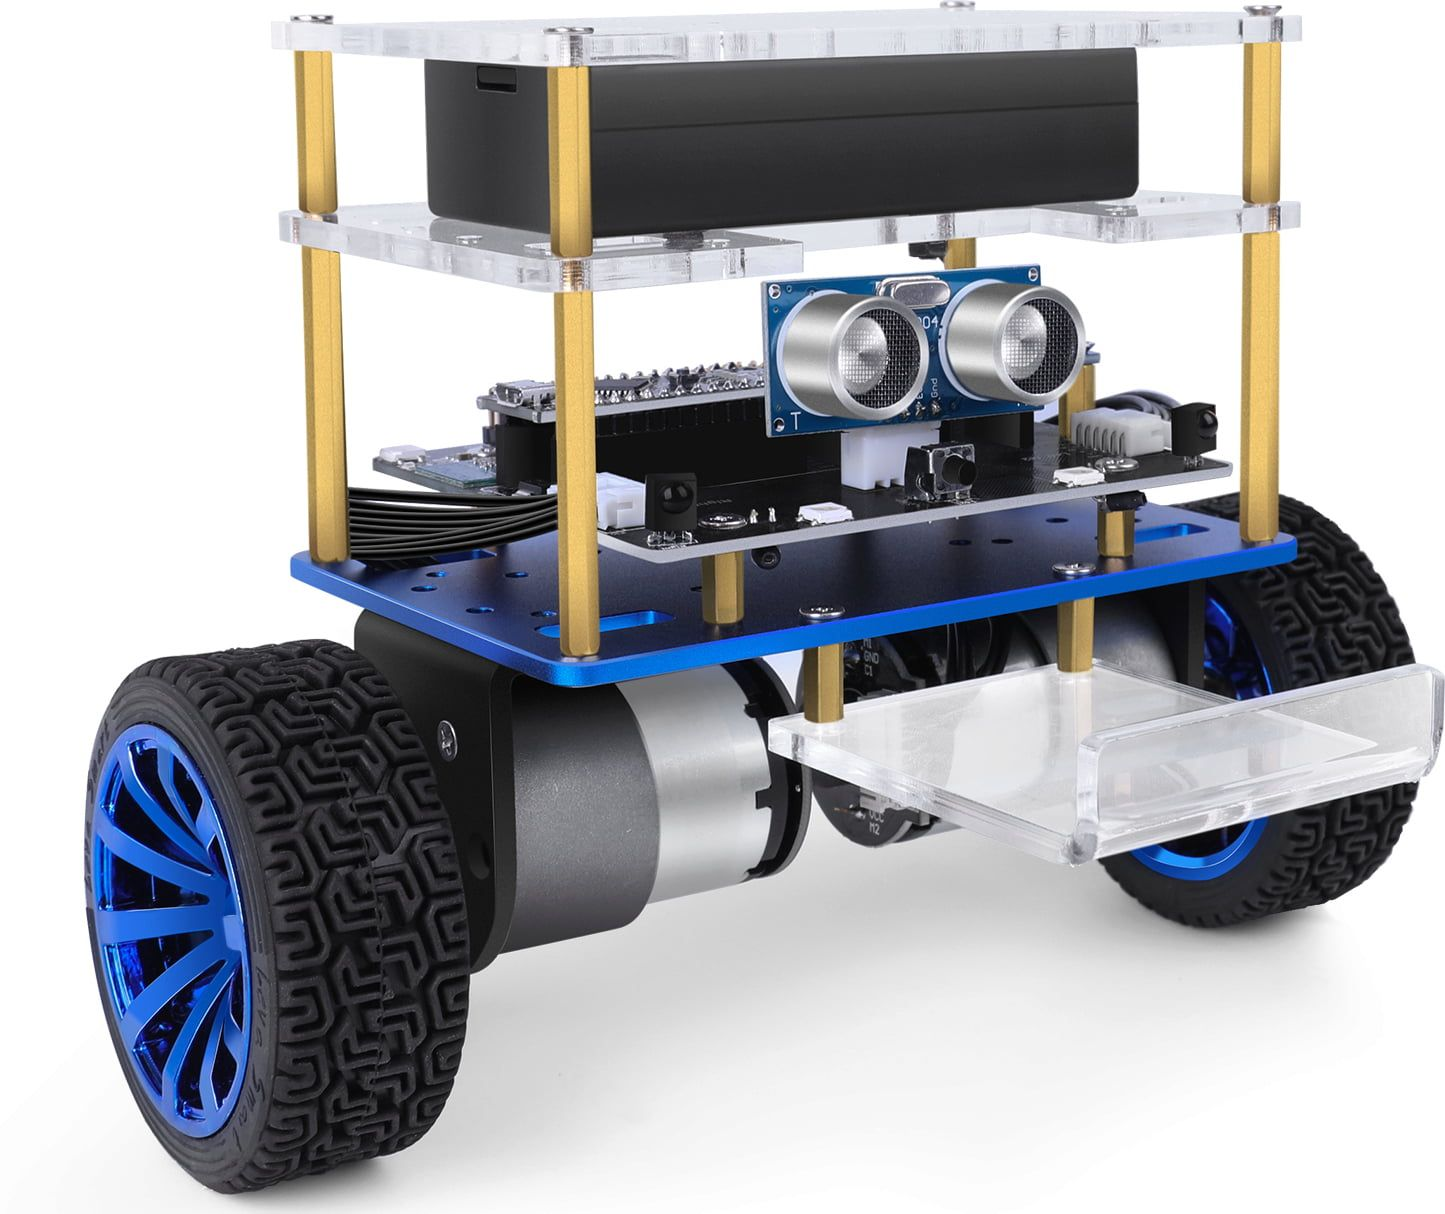
\includegraphics[height=6cm]{assets/tumbller.jpg}
	\caption{\label{fig:tumbler} ELEGOO Tumbler which was used for this project \cite{tumbller}.}
\end{figure}

\subsection{Project Objectives}
The primary objectives of this project are as follows:
\begin{itemize}
	\item To design and implement a two-wheeled self-balancing robot capable of maintaining stability using sensor feedback and control algorithms.
	\item To develop a cascaded PID control system for real-time balance and motion control, ensuring robustness and responsiveness.
	\item To integrate an MPU6050 inertial measurement unit (IMU) for accurate state estimation, utilizing sensor fusion techniques such as a Kalman filter.
	\item To enable remote monitoring and control of the robot, enhancing its versatility for various applications.
	\item To document the design, implementation, and tuning processes, providing a comprehensive resource for future development and replication.
\end{itemize}


\section{Literature Review}
Two-wheeled self-balancing robots have been widely studied as a variant of the classic inverted pendulum problem, requiring advanced control strategies to maintain stability. Various approaches, including Proportional-Integral-Derivative (PID) control \cite{matlab_inverted_pendulum}, Linear Quadratic Regulator (LQR)~\cite{10193276} have been explored to achieve robust balancing and motion control.

Xu and Duan~\cite{1174486} demonstrated that the Linear Quadratic Regulator (LQR) controller outperforms the pole-placement controller in both simulation and real-time control scenarios.

Kalman filtering has been extensively used for sensor fusion in such systems, particularly for integrating accelerometer and gyroscope data to obtain accurate state estimates. Studies have demonstrated that complementary and extended Kalman filters significantly improve stability and noise rejection in sensor-driven control systems.

Recent advancements in autonomous navigation for self-balancing robots have incorporated Simultaneous Localization and Mapping (SLAM) techniques, LiDAR-based obstacle detection, and machine learning-based adaptive control methods \cite{Tsai_Chih_2008} \cite{Ranasinghe_Vidanapathirana_2019}. These improvements enable real-time path planning and environmental interaction, making self-balancing robots more suitable for real-world applications such as personal mobility, surveillance, and industrial automation.

This project builds upon these existing methodologies by implementing a Kalman filter for sensor fusion and employing PID-based control to achieve stable balancing and maneuverability. Future work aims to integrate more advanced control and navigation techniques for enhanced autonomy and performance.

\subsection{Scope of Work}
The scope of this project encompasses the following key areas:
\begin{itemize}
	\item \textbf{Hardware Integration:} Assembling and configuring the ELEGOO Tumbler platform, including the MPU6050 IMU, motor drivers, and encoders.
	\item \textbf{Software Development:} Implementing firmware for the Arduino Nano microcontroller using PlatformIO, focusing on sensor data acquisition, control algorithms, and communication protocols.
	\item \textbf{Control System Design:} Designing and tuning a cascaded PID control loop for pitch, yaw, and position control, ensuring stable and precise operation.
	\item \textbf{Sensor Fusion:} Utilizing a Kalman filter to fuse data from the IMU, improving the accuracy of state estimation and control.
	\item \textbf{Testing and Validation:} Conducting extensive testing to evaluate the robot's performance under various conditions, followed by iterative refinement of the control parameters.
	\item \textbf{Documentation and Open-Source Contribution:} Providing detailed documentation, including schematics, code, and tuning guidelines, and making the project available on a \href{https://github.com/haris-mujeeb/Self-Balancing-Robot}{GitHub repository} for open-source collaboration \cite{opensource}.
\end{itemize}

\begin{figure}[h]
	\centering
	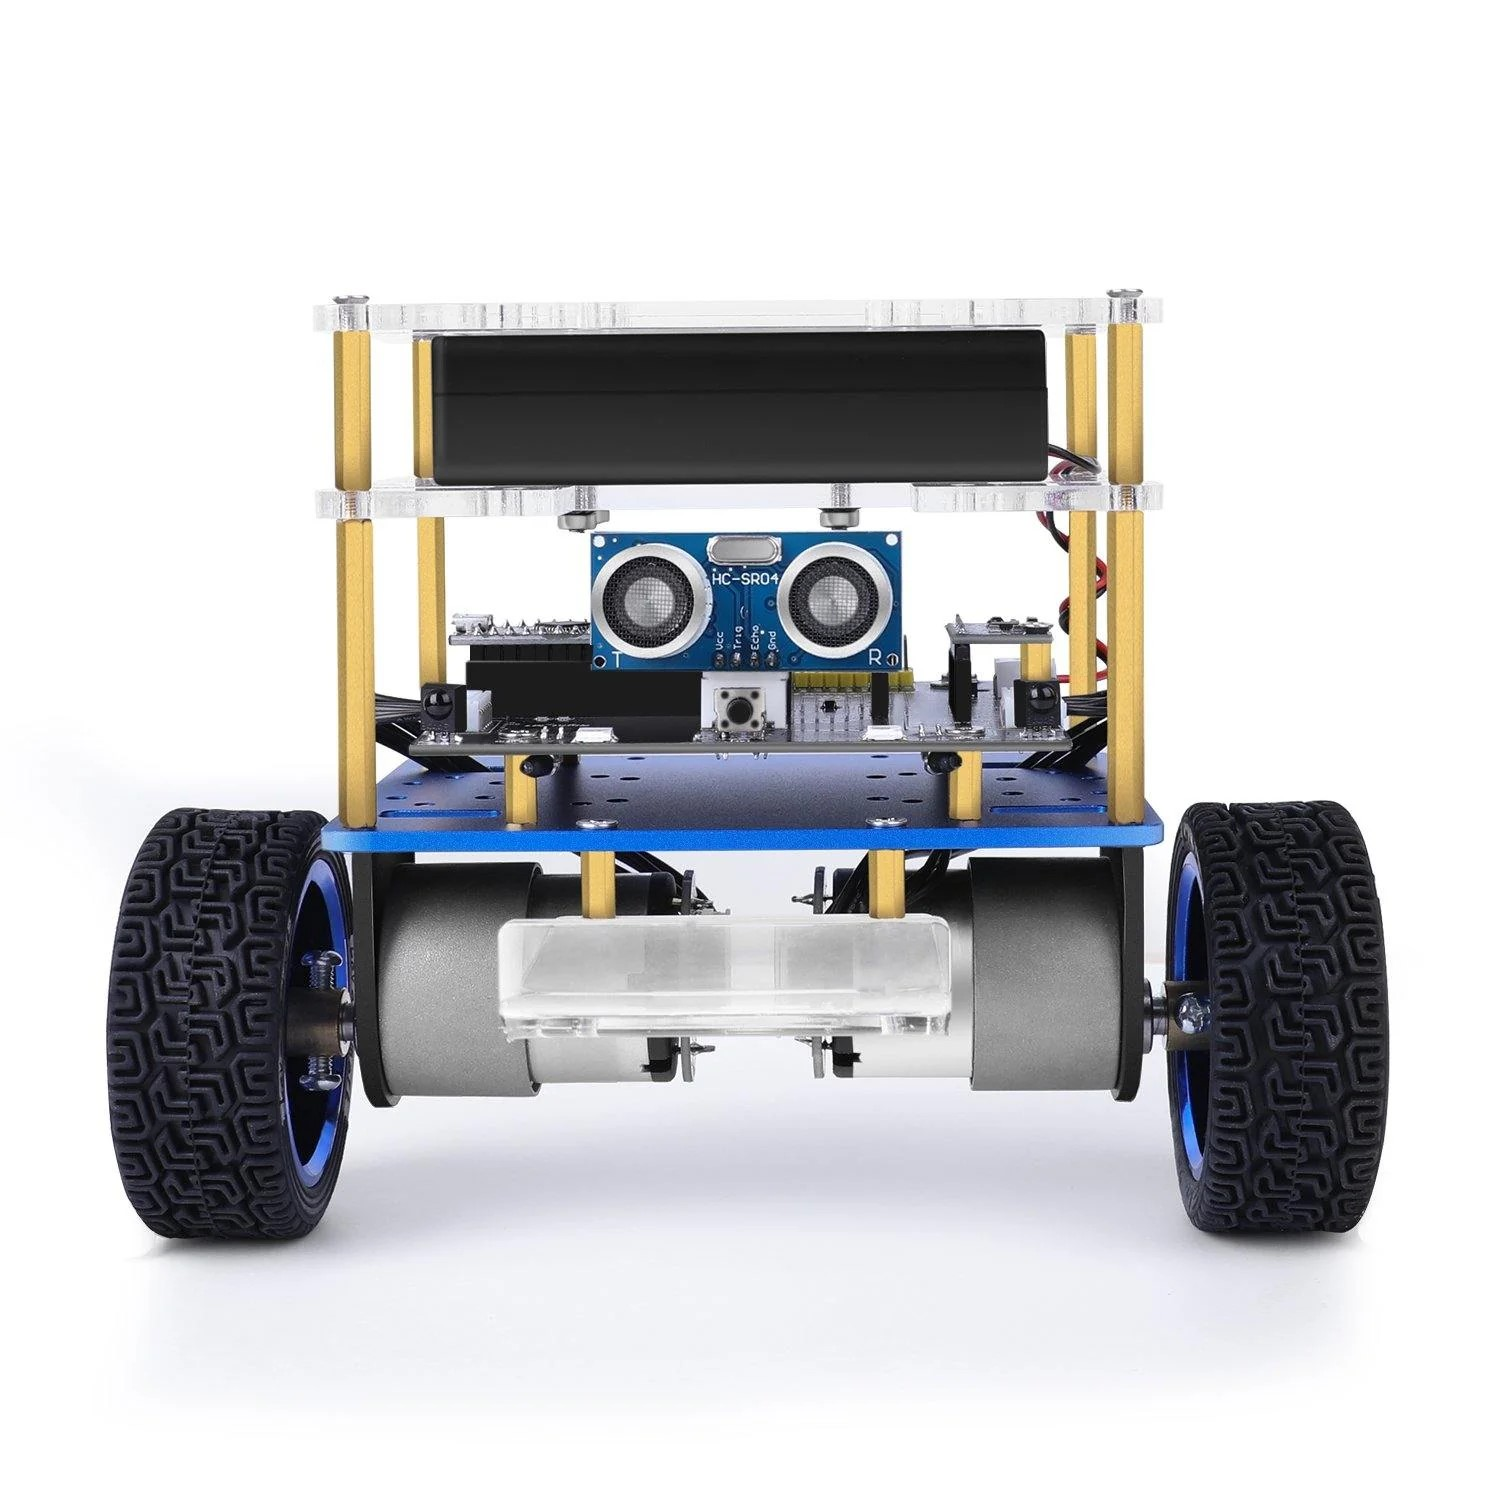
\includegraphics[height=6cm]{assets/tumbller2.jpg}
	\caption{\label{fig:tumbler2} ELEGOO Tumbler \cite{tumbller}.}
\end{figure}
	

\section{Mathematical Modelling}
$$
\begin{bmatrix}
    \dot{x} \\
    \ddot{x} \\
    \dot{\psi} \\
    \ddot{\psi}
\end{bmatrix}
= A
\begin{bmatrix}
    x \\
    \dot{x} \\
    \psi \\
    \dot{\psi}
\end{bmatrix}
+ B u_{input}
$$

	\subsection{Software Implementation Overview} \label{sec:software_overview}
Figure~\ref{fig:code-overview-flowchart} illustrates the overall system architecture and control flow.
\begin{figure}[h]
	\centering
	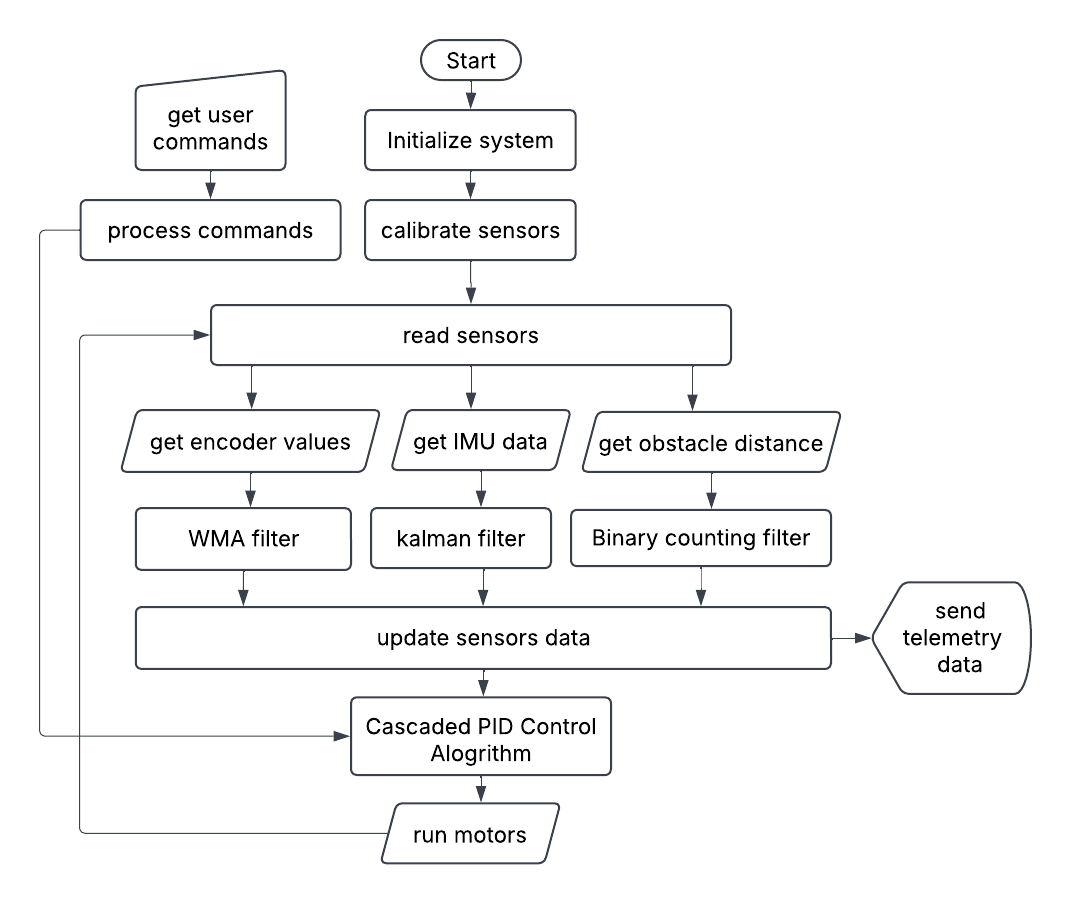
\includegraphics[width=0.8\linewidth]{assets/code_overview_flowchart.png}
	\caption{System operational flowchart.}
	\label{fig:code-overview-flowchart}
\end{figure}

The process begins with the reception of user commands, which are then parsed and processed.  Subsequently, the system initializes and calibrates its various sensors.  Sensor data, including encoder values, IMU data, and obstacle distance, is acquired and passed through respective filters (WMA, Kalman, and Binary Counting) to reduce noise and improve accuracy.  The filtered sensor data is then aggregated and used to update the robot's internal state.

\begin{figure}[h]
	\centering
	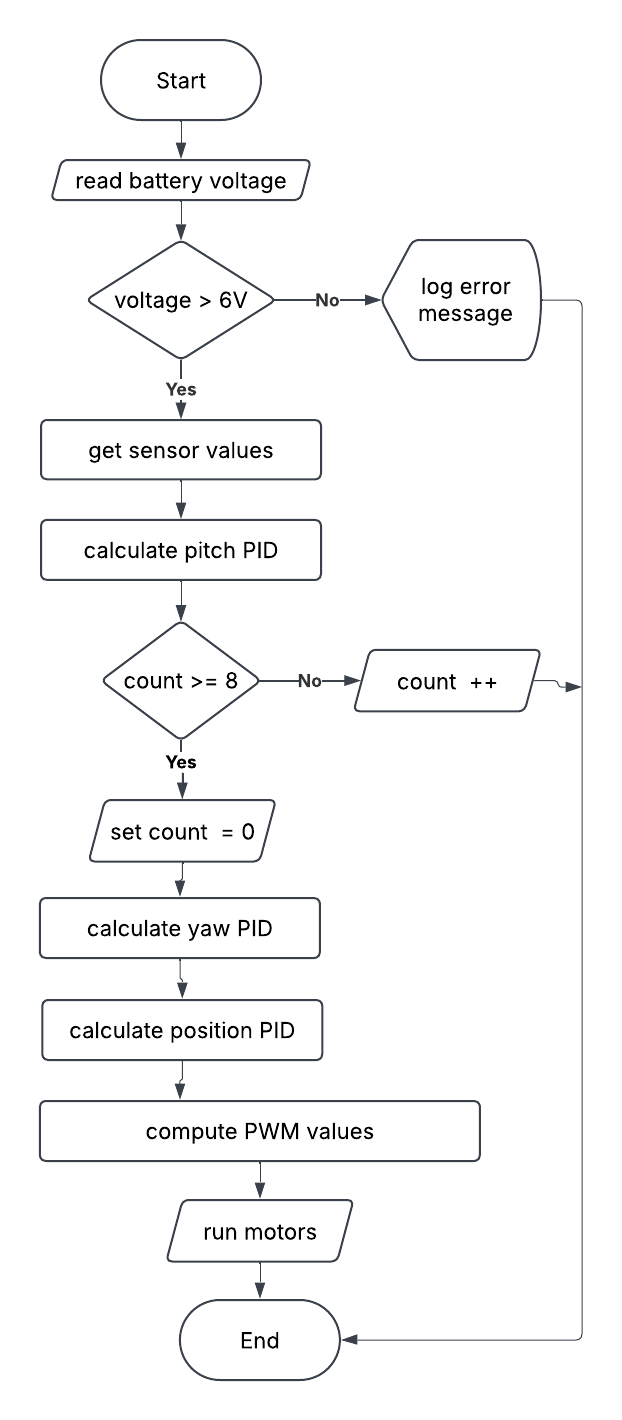
\includegraphics[width=0.5\linewidth]{assets/control_loop_diagram.png}
	\caption{A simplified block diagram of the cascaded control loop used. }
	\label{fig:control-loop}
\end{figure}

To stabilize the inverted pendulum in the upright position and to control the robot at the desired position using the PID control approach, two PID controllers with Linear–quadratic regulator (LQR) control : Yaw angle PID controller and position PID controller have been designed for the two control loops of the system.

A cascaded PID control algorithm (shown in Fig.~\ref{fig:control-loop}) utilizes the updated sensor data to calculate appropriate motor commands. These commands are then sent to the motors, driving the robot's movement.  Throughout this process, telemetry data is generated and transmitted, providing feedback on the robot's status and performance.  This closed-loop control and monitoring system ensures precise and reliable operation. Further details on the individual components and algorithms are provided in the following subsections.
	\section{Sensor Fusion for Self-Balancing Robot using MPU6050}
\subsection{Introduction}
Self-balancing robots require accurate estimation of their tilt angle for effective control. The MPU6050, a widely used Inertial Measurement Unit (IMU), provides raw accelerometer and gyroscope data. However, due to individual sensor limitations, direct usage of these readings is unreliable. Sensor fusion techniques like the Complementary Filter and Kalman Filter help in obtaining a stable and accurate tilt angle

\subsubsection{Microcontroller}
The ATmega328P (shown in Fig. \ref{fig:ATmega328p}) is a popular microcontroller from Microchip Technology, widely used in embedded systems and electronics projects. With a 16 MHz clock speed, 32 KB of flash memory, 2 KB of SRAM, and 1 KB of EEPROM \cite{atmega_microchip}, the ATmega328P provides ample resources for this projects application. 

The ATMEGA328P is also used in the Arduino Nano (shown in Fig. \ref{fig:arduino_nano}), a widely adopted development board known for its low cost and open-source ecosystem \cite{arduino_nano}. The combination of affordability and extensive community support makes it an ideal choice for rapid prototyping and academic research, ensuring easy integration with various sensors and motor drivers. 

\begin{figure}[H]
	\centering
	\subfloat[ATMEGA328P \cite{atmega_microchip}.]{
		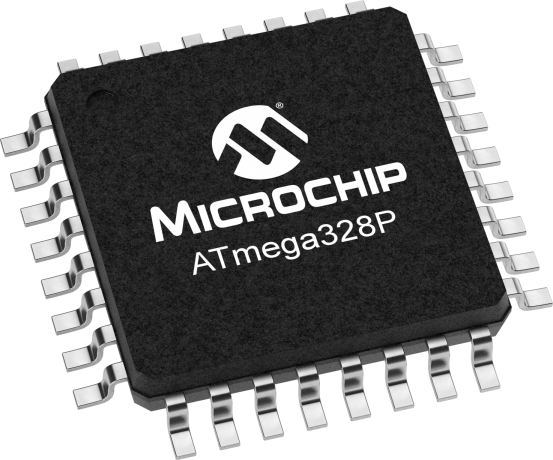
\includegraphics[height=3cm]{assets/ATmega328p.png}
		\label{fig:ATmega328p}
	}
	\qquad
	\subfloat[Arduino Nano \cite{arduino_nano}.]{
	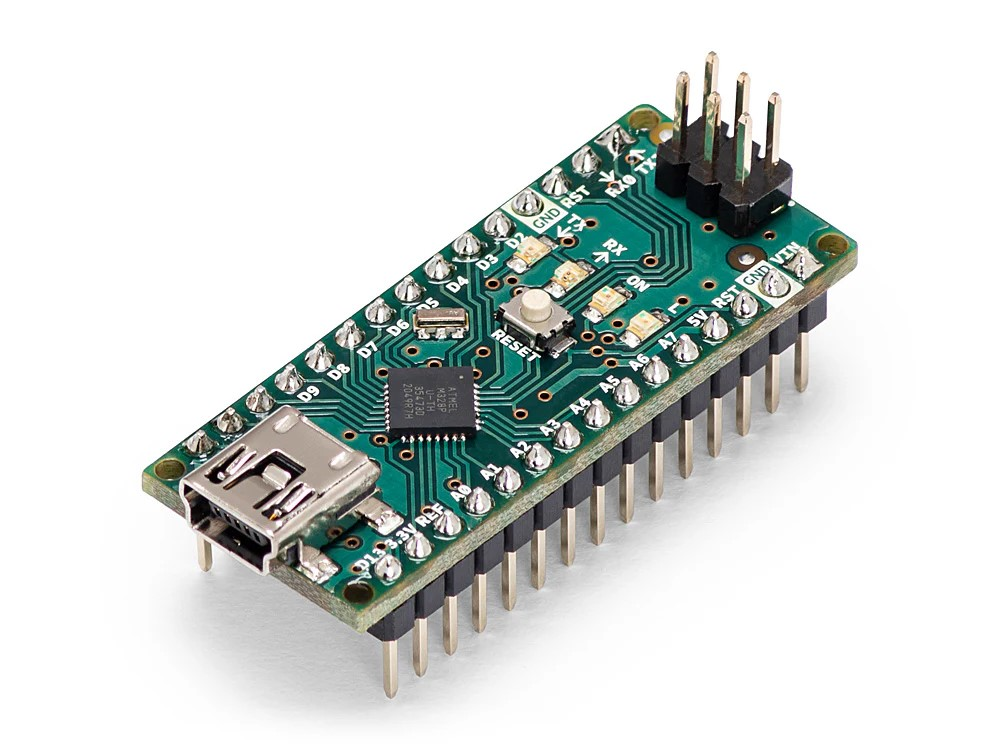
\includegraphics[height=3cm]{assets/arduino_nano.jpg}
	\label{fig:arduino_nano}
	} 
	\label{fig:ATmega328p_and_arduino_nano}
	\caption{}
\end{figure}

\subsubsection{Inertial Measuring Unit}
The MPU6050 is a widely used six-axis sensor that integrates a three-axis gyroscope and a three-axis accelerometer on a single chip, making it essential for motion tracking and stabilization applications (shown in Fig. \ref{fig:mpu-6050}). Its compact design and built-in Digital Motion Processor (DMP) enable real-time processing of sensor data, which is crucial for robotics, drones, and wearable devices.
In applications like self-balancing robots, it provides accurate orientation and acceleration data necessary for maintaining stability. 

\begin{figure}[H]
	\centering
	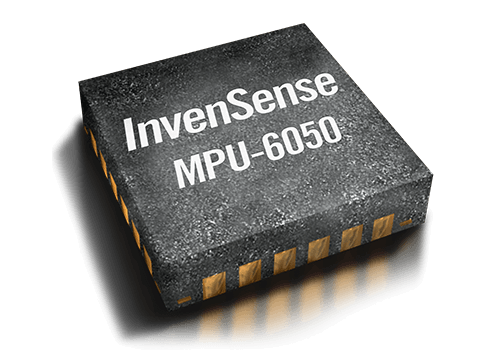
\includegraphics[height=3cm]{assets/mpu-6050.png}
	\caption{MPU-6050 \cite{mpu6050}.}
	\label{fig:mpu-6050}
\end{figure}


\subsection{Working of MPU6050}
The MPU6050 is a 6-axis IMU that provides:
\begin{itemize}
	\item Accelerometer Data: Measures acceleration in X, Y, and Z axes. It helps in estimating tilt based on gravitational force.
	\item Gyroscope Data: Measures angular velocity around X, Y, and Z axes. Integration of gyroscope readings over time provides the tilt angle.
\end{itemize}

\subsubsection{Reading Raw Sensor Data}
The \texttt{read\_mpu\_6050\_data()} function reads raw data from the MPU6050 sensor:
\begin{itemize}
	\item It requests 14 bytes of data from the sensor, covering the accelerometer, gyroscope, and temperature sensor readings.
	\item The data is stored in respective variables after combining the high and low bytes. 
	\item If data retrieval fails, an error message is displayed.
\end{itemize}
\begin{lstlisting}[style=cppstyle2]
void mpu6050Base::read_mpu_6050_data() {
	Wire.beginTransmission(mpu6050_addr);
	Wire.write(0x3B);
	Wire.endTransmission();
	Wire.requestFrom(mpu6050_addr, (uint8_t)14);
	
	if (Wire.available() >= 14) {
		acc_x = Wire.read() << 8 | Wire.read();
		acc_y = Wire.read() << 8 | Wire.read();
		acc_z = Wire.read() << 8 | Wire.read();
		temperature = Wire.read() << 8 | Wire.read();
		gyro_x = Wire.read() << 8 | Wire.read();
		gyro_y = Wire.read() << 8 | Wire.read();
		gyro_z = Wire.read() << 8 | Wire.read();
	} else {
		ERROR_PRINT("Data cannot be read from MPU6050!");
	}
	
}
\end{lstlisting}

\subsubsection{Issues with Raw Sensor Data}
\begin{itemize}
\item \textbf{Accelerometer Noise}: While providing an absolute angle reference, accelerometer readings are noisy and susceptible to external forces.
\item \textbf{Gyroscope Drift}: Over time, integration errors cause drift, leading to inaccurate angle estimation.
To overcome these issues, sensor fusion techniques are applied.
\end{itemize}


\subsection{Complementary Filter}
The complementary filter is a simple yet effective method for sensor fusion \cite{rabbany_design_2021} \cite{10193276} \cite{1174486}. It blends high-frequency data from the gyroscope with low-frequency data from the accelerometer:

\subsubsection{Mathematical Model}
Raw accelerometer readings $A_y$ and $Az$ can be used to calculate tilt angle using following equation:
\begin{equation}
\theta_{acc} = \text{arctan} \left(A_y/Az  \right) \label{eq:eq}
\end{equation}
Similarly, using raw angular velocity data from the gyroscope $\omega_{x}$,
\begin{equation}
	\begin{aligned}
		\dot{\theta}_{gyro}(t) &= - \omega_{x,bias}(t) \\ \label{eq:state_eq_1}
		\dot{\omega}_{x,bias}(t) &= 0
	\end{aligned}
\end{equation}
In these equations, $\theta(t)$ represents the measured angle of the system, and $\omega_{\text{gyro,bias}}(t)$ represents the bias of the gyroscope. The first equation models how the angle evolves over time, influenced by the constant gyroscope bias. The second equation indicates that the gyroscope bias remains constant over time. The sampling time interval $\Delta t$ and previous angle value $\theta_{previous}$ can be used to calculate tilt angle using following equation:
\begin{equation}
\theta_{gyro} = \theta_{previous, gyro} + \omega_{gyro} \Delta t \label{eq:eq}
\end{equation}
Then the final estimated angle $\theta_{estimate}$ is calculated as:
\begin{equation}
	\theta_{estimate} = \alpha \ \theta_{gyro} + (1 - \alpha) \ \theta_{acc} \label{eq:eq}
\end{equation}
Where $\alpha$ is the filter coefficient, $\omega$ is the angular velocity from the gyroscope, and $\theta_{acc}$ is the angle from the accelerometer.

\subsubsection{Initial Calibration}
The \texttt{init()} function is responsible for initializing the MPU6050 sensor and performing gyroscope calibration:
\begin{itemize}
	\item The I2C communication is established with the sensor, and an acknowledgment is checked to ensure proper connection.
	\item The function sets up the MPU6050 registers using \texttt{setup\_mpu\_6050\_registers()}, configuring the power management and sensitivity ranges for both the accelerometer and gyroscope.
	\item Gyroscope calibration is performed by collecting multiple readings and averaging them to calculate offsets for the X, Y, and Z axes. These offsets help reduce sensor drift.
\end{itemize}

\begin{lstlisting}[style=cppstyle2]
void mpu6050Base::init() {
	Wire.beginTransmission(mpu6050_addr);
	if (Wire.endTransmission() != 0) {
		ERROR_PRINT("MPU6050 not connected!");
		return;
	}
	setup_mpu_6050_registers();
	
	for (int i = 0; i < CALIBRATION_SAMPLES; i++) {
		read_mpu_6050_data();
		gyro_x_cal += gyro_x;
		gyro_y_cal += gyro_y;
		gyro_z_cal += gyro_z;
		delay(3);
	}
	gyro_x_cal /= CALIBRATION_SAMPLES;
	gyro_y_cal /= CALIBRATION_SAMPLES;
	gyro_z_cal /= CALIBRATION_SAMPLES;
}
\end{lstlisting}

\subsubsection{Calculating Angles}
The \texttt{calculate()} function processes raw sensor data to determine pitch and roll angles:
\begin{itemize}
	\item Gyroscope readings are corrected using calibration offsets to remove bias.
	\item Angular velocity is integrated over time to estimate orientation changes.
	\item The accelerometer-derived angles are computed from the total acceleration vector using trigonometric transformations.
	\item A complementary filter is applied to blend gyroscope and accelerometer readings, mitigating drift and noise while enhancing stability.
\end{itemize}

\begin{lstlisting}[style=cppstyle2]
void mpu6050Base::calculate() {
	read_mpu_6050_data();
	
	gyro_x -= gyro_x_cal;
	gyro_y -= gyro_y_cal;
	gyro_z -= gyro_z_cal;
	
	angle_pitch += gyro_x * 0.0000611;
	angle_roll += gyro_y * 0.0000611;
	
	angle_pitch += angle_roll * sin(gyro_z * 0.000001066);
	angle_roll -= angle_pitch * sin(gyro_z * 0.000001066);
	
	acc_total_vector = sqrt((acc_x * acc_x) + (acc_y * acc_y) + (acc_z * acc_z));
	
	angle_pitch_acc = asin((float)acc_y / acc_total_vector) * 57.296;
	angle_roll_acc = asin((float)acc_x / acc_total_vector) * -57.296;
	
	if (set_gyro_angles) {
		angle_pitch = angle_pitch * 0.9996 + angle_pitch_acc * 0.0004;
		angle_roll = angle_roll * 0.9996 + angle_roll_acc * 0.0004;
	} else {
		angle_pitch = angle_pitch_acc;
		angle_roll = angle_roll_acc;
		set_gyro_angles = true;
	}
	
	angle_pitch_output = angle_pitch_output * 0.9 + angle_pitch * 0.1;
	angle_roll_output = angle_roll_output * 0.9 + angle_roll * 0.1;
	
}
\end{lstlisting}


\subsubsection{Results}

\begin{figure}[H]
	\centering
	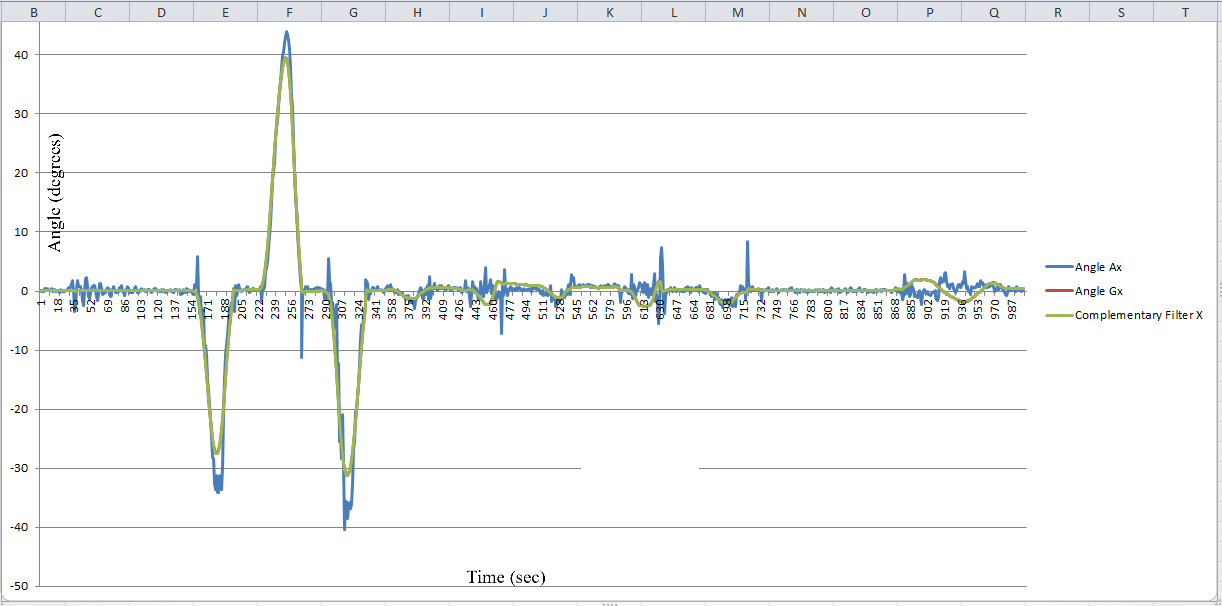
\includegraphics[height=8cm]{assets/compl_filter_0.9.png}
	\caption{Pitch angle caluclated using a complementary filter with $\omega = 0.9$.}
	\label{fig:battery}
\end{figure}

	
\subsection{Extended Kalman Filter (EKF)}
The Kalman filter (KF) provides a more sophisticated approach, estimating the true state of the system by minimizing the mean of the squared error. It involves prediction and update steps. However,  assumes that both the process and measurement models are linear. However, many real-world systems, such as robotic motion and sensor fusion, exhibit inherent nonlinearities. When linearization is not feasible, the standard KF becomes inaccurate. 

To address this limitation, the Extended Kalman Filter (EKF) extends the KF to nonlinear systems by employing a first-order Taylor series expansion. This method approximates the nonlinear system dynamics and measurement models with locally linearized representations, allowing the filter to be applied in scenarios where exact linearization is not feasible.

The EKF is an extension of the Kalman Filter for nonlinear systems, utilizing first-order Taylor series expansion to linearize process and measurement models. EKF maintains a Gaussian belief over the state, updating it through a prediction-correction cycle. The Jacobian matrices of the system dynamics and measurement functions are used to approximate state transitions and measurement updates. Its advantages include handling nonlinearities, fusing multi-sensor data, and improving estimation accuracy in noisy environments. 

\subsubsection{General State Equation}
For non-linear system, with Stochastic disturbances:
\begin{equation}
\begin{aligned}
	\dot{\underline{x}}(t) &= f\left( \underline{x}(t), \underline{u}(t) \right) + \underline{d}(t) \\
	\underline{y}(t) &= h\left( \underline{x}(t) \right) + \underline{n}(t)
\end{aligned}
\end{equation}
where,
\begin{itemize}
	\item $ \dot{\underline{x}}(t) $: This represents the time derivative of the state vector $ \underline{x}(t) $, indicating how the state evolves over time.
	\item $ f $: This is a nonlinear function that describes the system dynamics, taking the current state $ \underline{x}(t) $ and the control input $ \underline{u}(t) $ as arguments. It captures how the state changes based on the current state and control inputs.
	\item $ \underline{d}(t) $: This term represents stochastic disturbances (or process noise) affecting the state dynamics, typically modeled as a zero-mean Gaussian noise.
	\item $ y(t) $: This is the measurement vector at time $ t $, representing the observed outputs of the system. It is the data collected from sensors or measurement devices.
	\item $ h $: This is a nonlinear measurement function that maps the true state vector $ \underline{x}(t) $ to the measurement space. It describes how the state influences the measurements. The function $ h $ can be complex and may involve various transformations of the state variables.
	\item $ n(t) $: This term represents measurement noise, which is also typically modeled as zero-mean Gaussian noise. It accounts for inaccuracies in the measurements due to sensor errors, environmental conditions, or other random factors that can affect the observed data.
\end{itemize}

\subsubsection{State Estimation}
For a non-linear system the state form is as follows,
\begin{equation}
\begin{aligned}
	\dot{\hat{\underline{x}}}(t) &= f\left( \underline{\hat{x}}(t), \underline{u}(t) \right) + \underline{K}\left( y(t) - \hat{y}(t) \right) \\
	\hat{y}(t) &= h\left( \underline{\hat{x}}(t) \right)  \label{eq:eq}
\end{aligned}
\end{equation}
The Kalman gain $\underline{K}$ is computed to optimally balance estimation uncertainty and measurement noise. To achieve this, the system is first linearized around the current state estimate by computing the Jacobians of the process and measurement models. To linearize the system around the current state estimate, the Jacobian matrices, which represent the first-order partial derivatives of the nonlinear functions, are computed as follows:
\begin{equation}
\underline{A}(t) = \frac{\mathrm{d}f}{\mathrm{d}\underline{x}} \bigg|_{\underline{\hat{x}}(t), \underline{u}(t)} \quad \text{and} \quad
\underline{C}(t) = \frac{\mathrm{d}h}{\mathrm{d}\underline{x}} \bigg|_{\underline{\hat{x}}(t)}  \label{eq:eq}
\end{equation}
where $\underline{A}(t)$ represents the partial derivatives of the state dynamics function $f$ and $\underline{C}(t)$ represents the partial derivatives of the measurement function $h$.
\begin{figure}[h]
	\centering
	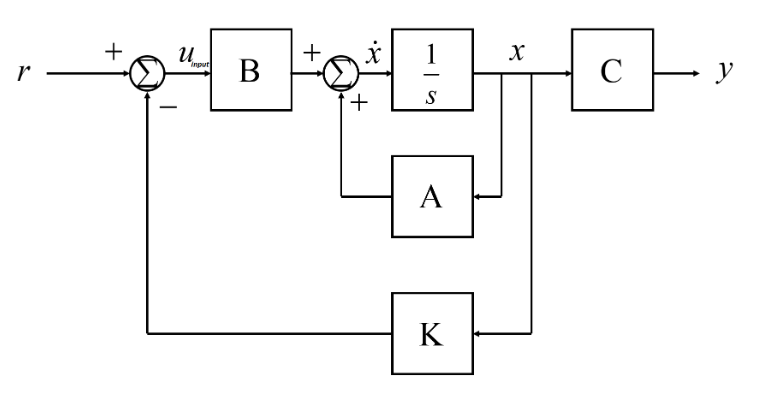
\includegraphics[height=5cm]{assets/block_representation_kalman_filter.png}
	\caption{Block representation of state space system showing the system matrices $A$, $B$ and $C$ as well as the gain matrix $K$.}
	\label{fig:block_representation_kalman_filter}
\end{figure}
\subsubsection{Covraince Matrix}
The evolution of the state estimation covariance matrix follows the continuous-time Riccati equation, given by:
\begin{equation}
\dot{P}(t) = \underline{A}(t) P(t) + P(t) \underline{A}^T(t) + Q - P(t) \underline{C}^T(t) R^{-1} \underline{C}(t) P(t)  \label{eq:eq}
\end{equation}
Where, 
\begin{itemize}
	\item $\dot{P}(t)$: his represents the time derivative of the covariance matrix $\dot{P}(t)$, which quantifies the uncertainty in the state estimate over time.
	\item $\underline{A}(t)$: This is the state transition matrix, which describes how the state evolves from one time step to the next.
	\item $Q$: This is the process noise covariance matrix, representing the uncertainty in the process model.
	\item $\underline{C}(t)$: This is the measurement matrix, which relates the state to the measurements.
	\item $R$: This is the measurement noise covariance matrix, representing the uncertainty in the measurements.
\end{itemize}
The Kalman filter is initialized with an initial covariance matrix:
\begin{equation}
	P(0) = \mathbf{E}(\Delta\underline{x}(0) \Delta\underline{x}^T(0))  \label{eq:eq}
\end{equation}
The optimal Kalman gain, balancing estimation uncertainty and measurement noise, is given by:

\begin{equation} \underline{K}(t) = P(t) \underline{C}^T R^{-1} \end{equation}
The time-discrete Kalman filter state update equations are:
\begin{equation}
	\begin{aligned}
		\underline{x}_{k} &= \underline{A} \underline{x}_{k-1} + \underline{B} \underline{u}_{k} + \underline{d}_{k-1} \\
		\underline{y}_{k} &= \underline{C} \underline{x}_{k} + \underline{n}_{k}  \label{eq:eq}
	\end{aligned}
\end{equation}
where $\underline{x}_k$ is the state vector, $\underline{B}$ the control input matrix, and $\underline{y}_k$ the measurement vector. The discrete state-space representation is:
\begin{equation}
	\begin{aligned}
		\underline{\dot{x}}(t) = \underline{A}.\underline{x}(t) + \underline{B}.\underline{u}(t) \\
		\underline{y}(t) = \underline{C}.\underline{x}(t) + \underline{D}.\underline{u}(t)  \label{eq:eq}
	\end{aligned}
\end{equation}
The state covariance matrix is:
\begin{equation}
	\mathbf{P}_k = \begin{bmatrix} P_{00} & P_{01} \\ P_{10} & P_{11} \end{bmatrix}  \label{eq:eq}
\end{equation}
where $P_{00}$ represents uncertainty in the angle estimate and $P_{11}$ in gyroscope bias. The Kalman gain is computed as:
\begin{equation}
	\begin{aligned}
		\underline{K}_{k} &= \underline{P}_{k}^- \ \underline{C}^T ( \underline{C} \ \underline{P}_{k}^-\ \underline{C}^T  +\underline{R})^{-1} \\ \\
		\mathbf{K}_k &= \begin{bmatrix} \frac{ P_{00} }{ P_{00}  
				+ R_{angle}} \\ \frac{ P_{10} }{ P_{00}  
				+ R_{angle}} \end{bmatrix}
	\end{aligned}  \label{eq:eq}
\end{equation}
Following the prediction step, the measurement update step refines the state estimate using the Kalman gain, which is derived to minimize the posterior estimation error covariance (see Appendix \ref{appendix:B} for detailed calculations):
\begin{equation}
	\begin{aligned}
		\underline{P}_{k} &= \ (\underline{I} - \underline{K}_{k} \ \underline{C}) \ \underline{P}_{k}^- \label{eq:eq}
	\end{aligned}
\end{equation}


\subsection{Software Implementation of EKF}
For the implementation of the Extended Kalman Filter (EKF), we utilized the Kalman filter library developed by Kristian Lauszus~\cite{github_kalman_filter}. This library was modified in accordance with the GNU General Public License to meet the specific requirements of our project.
\begin{lstlisting}[style=cppstyle2]
#include <Arduino.h>

class KalmanFilter {
 private:
  float m_dt, m_Q_angle, m_Q_gyro, m_R_angle, m_C_0;
  float q_bias = 0, angle_err = 0;
  float P[2][2] = {{1, 0}, {0, 1}}; // Covariance matrix
  float K_0 = 0, K_1 = 0;

 public:
  float angle = 0;

KalmanFilter(float dt, float Q_angle, float Q_gyro, float R_angle, float C_0)
: m_dt(dt), m_Q_angle(Q_angle), m_Q_gyro(Q_gyro), m_R_angle(R_angle), m_C_0(C_0) {}

float getAngle(float measured_angle, float measured_gyro) {
	// Predict
	angle += (measured_gyro - q_bias) * m_dt;
	angle_err = measured_angle - angle;
	
	// Update covariance matrix
	P[0][0] += m_Q_angle - P[0][1] - P[1][0];
	P[0][1] -= P[1][1];
	P[1][0] -= P[1][1];
	P[1][1] += m_Q_gyro;
	
	// Compute Kalman gain
	float E = m_R_angle + m_C_0 * P[0][0];
	K_0 = (m_C_0 * P[0][0]) / E;
	K_1 = (m_C_0 * P[1][0]) / E;
	
	// Update state
	angle += K_0 * angle_err;
	q_bias += K_1 * angle_err;
	
	// Update covariance matrix
	float C0_P00 = m_C_0 * P[0][0];
	P[0][0] -= K_0 * C0_P00;
	P[0][1] -= K_0 * P[0][1];
	P[1][0] -= K_1 * P[0][0];
	P[1][1] -= K_1 * P[0][1];
	
		return angle;
	}
};
\end{lstlisting}
	
\section{Motor Speed Control}
The system employs a cascaded Proportional-Integral-Derivative (PID) control loop to achieve real-time balance and motion control of the robot. This control architecture ensures stability by continuously monitoring and adjusting the robot's state using feedback from multiple sensors \cite{jamil_modeling_2014}. Key inputs to the control loop include:
the robot's pitch angle, gyroscope data, and motor encoder values, which provide critical information on orientation, angular velocities, and position. 
\begin{itemize}
	\item \textbf{Pitch angle}: Provides information about the robot's tilt relative to the vertical axis.
	\item \textbf{Gyroscope data}: Supplies angular velocity measurements for dynamic stabilization.
	\item \textbf{Motor encoder values}: Tracks wheel position and velocity for precise motion control.
\end{itemize}

The control algorithm computes outputs for \textbf{pitch}, \textbf{yaw}, and \textbf{position} at regular intervals, generating \textbf{pulse-width-modulation (PWM)} signals to adjust motor speeds via the motor driver (see Fig. \ref{fig:control-loop-block-diagram}). To prioritize system stability, the pitch angle is updated at a higher frequency (e.g., every control cycle), while the yaw angle and position control outputs are updated less frequently (e.g., every 8th cycle). This hierarchical approach ensures efficient resource utilization and robust performance.

\begin{figure}[H]
	\centering
	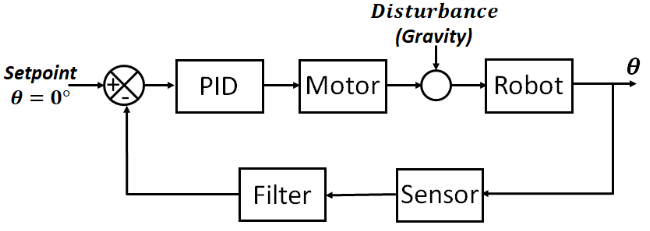
\includegraphics[height=3cm]{assets/control-loop-block-diagram}
	\caption{Robot's control block diagram.}
	\label{fig:control-loop-block-diagram}
\end{figure}
\subsubsection{Motor Driver}
The TB6612FNG dual motor driver (shown in Fig. \ref{fig:tb6612fng}) allows independent control of two DC motors. It uses a MOSFET H-bridge for bidirectional and Pulse Width Modulation (PWM) based motor speed control. Fig. \ref{fig:tb6612fng_plot} shows that each channel of the TB6612FNG can deliver up to 0.85A of current continuously. Furthermore, it consists of integrated over-current protection and thermal shutdown features for enhance reliability \cite{TB6612FNG}.

\begin{figure}[H]
	\centering
	\subfloat[TB6612FNG \cite{TB6612FNG_photo}.]{
		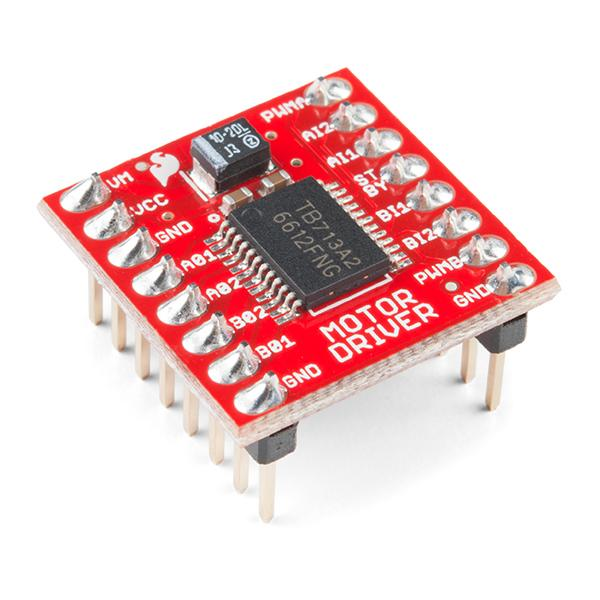
\includegraphics[height=3cm]{assets/TB6612FNG.jpg}
		\label{fig:tb6612fng}
	}\\ % Line break to stack the subfigures vertically
	\subfloat[Target characteristics for TB6612FNG \cite{TB6612FNG}.]{
		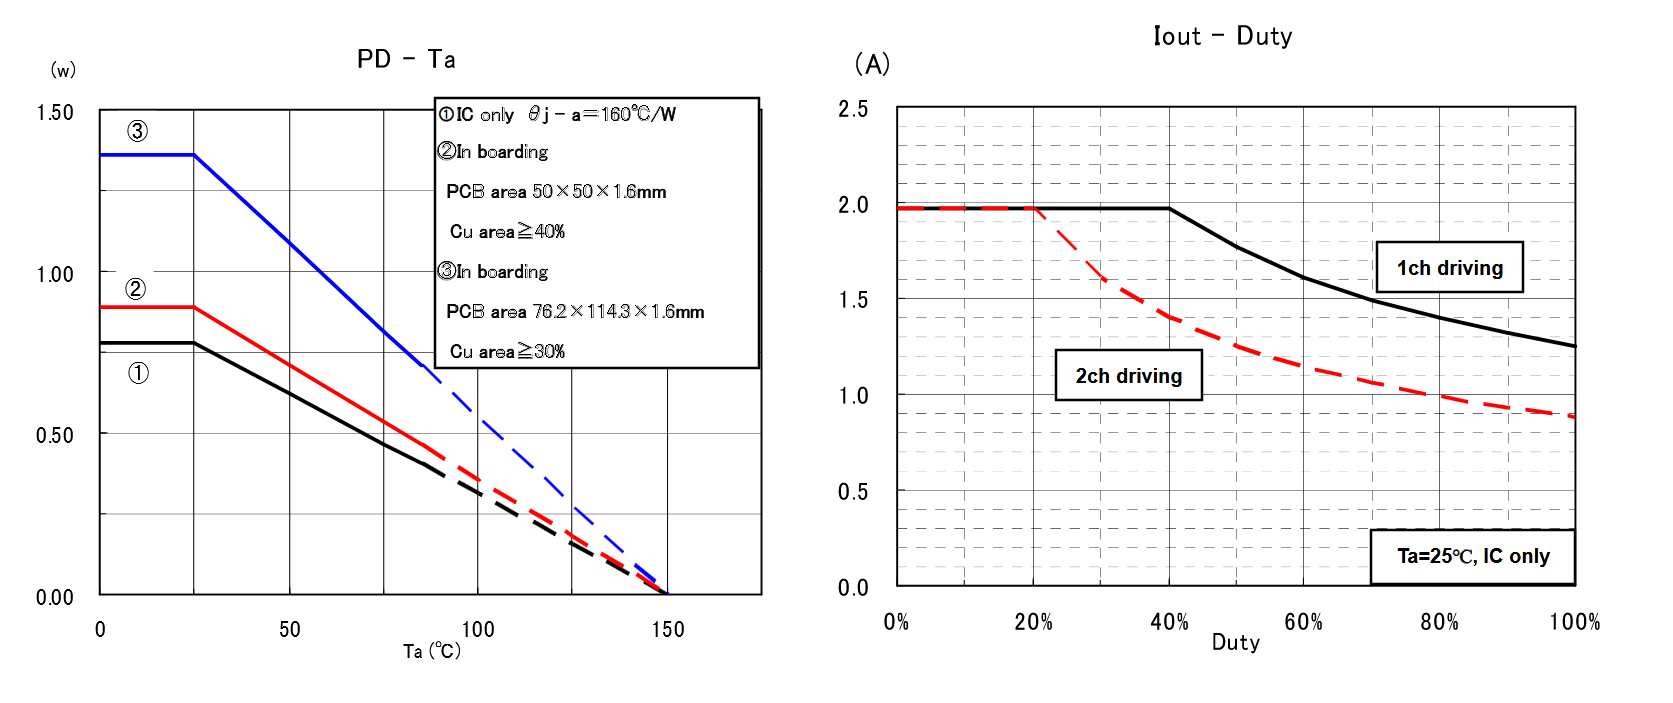
\includegraphics[height=6cm]{assets/TB6612FNG_target_characteristics}
		\label{fig:tb6612fng_plot}
	}
	\label{fig:tb6612fng_and_tb6612fng_plot}
	\caption{}
\end{figure}

Instead of using two separate MCU pins for direction control, a single pin can be used with an inverted Schmitt trigger to generate the complementary signal automatically. For this purspose SN74LVC2G14 (shown in Fig. \ref{fig:SN74LVC2G14}) is used. It also enhances motor control by improving signal stability (similar to what is shown in Fig. \ref{fig:schmitt_trigger_hysteresis}).  
\begin{figure}[H]
	\centering
	\subfloat[SN74LVC2G14 \cite{SN74LVC2G14}.]{
		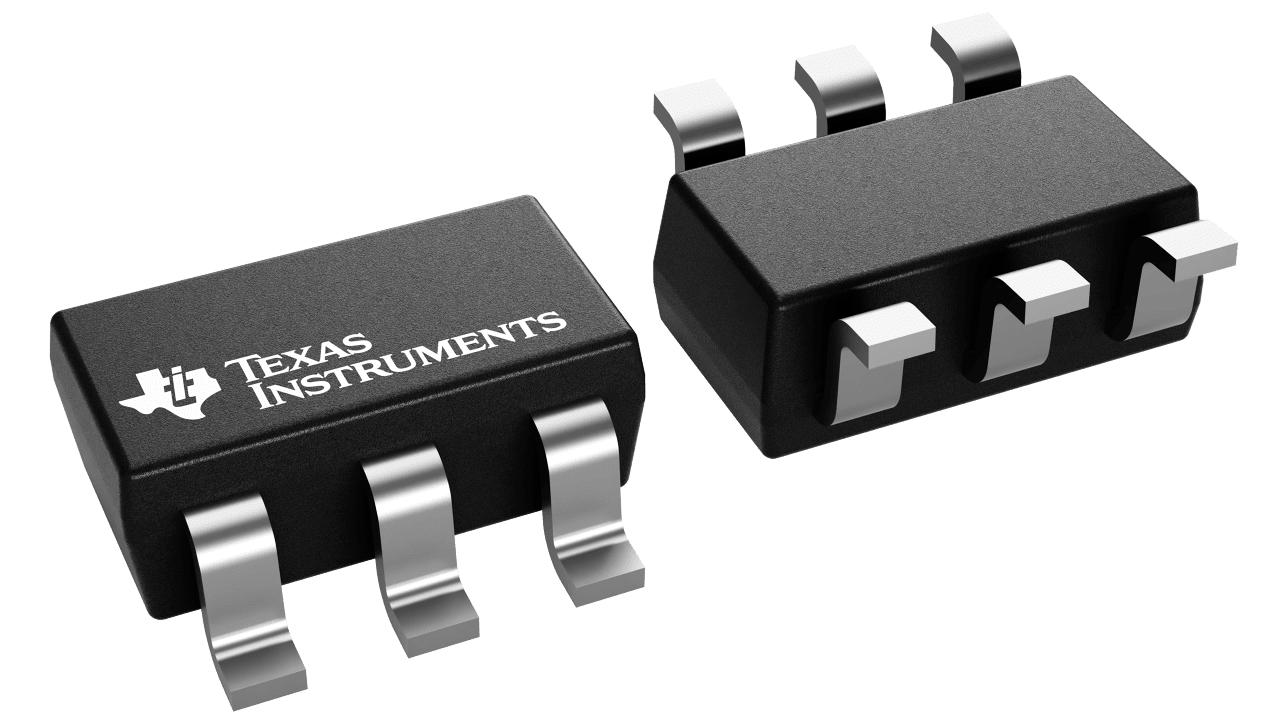
\includegraphics[height=2cm]{assets/SN74LVC2G14.png}
		\label{fig:SN74LVC2G14}
	}\\ % Line break to stack the subfigures vertically
	\subfloat[Schmitt trigger output without hysteresis (left) and with hysteresis (right) \cite{schmitt_trigger_hysteresis}.]{
		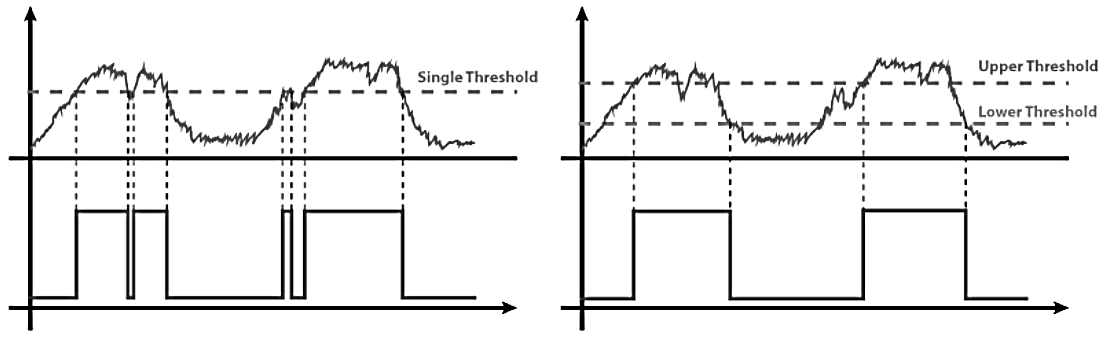
\includegraphics[height=4cm]{assets/schmitt_trigger_hysteresis.png}
		\label{fig:schmitt_trigger_hysteresis}
	}
	\label{fig:SN74LVC2G14_and_schmitt_trigger_hysteresis}	
	\caption{}
\end{figure}

\subsubsection{Drive Motors}
The drive system employs NNHYTECH GA37 520 DC motors (37mm diameter, 12V, 360 RPM) equipped with Hall effect encoders (shown in Fig. \ref{fig:dc-motor}) \cite{dc_motor}. These motors feature a reduction gearbox, which enhances torque output while maintaining controlled rotational speed, making them well-suited for applications requiring precise motion control. The Hall effect encoders generate quadrature signals, enabling accurate measurement of speed and position. Motors from NHYTech were in this case.
\begin{figure}[H]
	\centering
	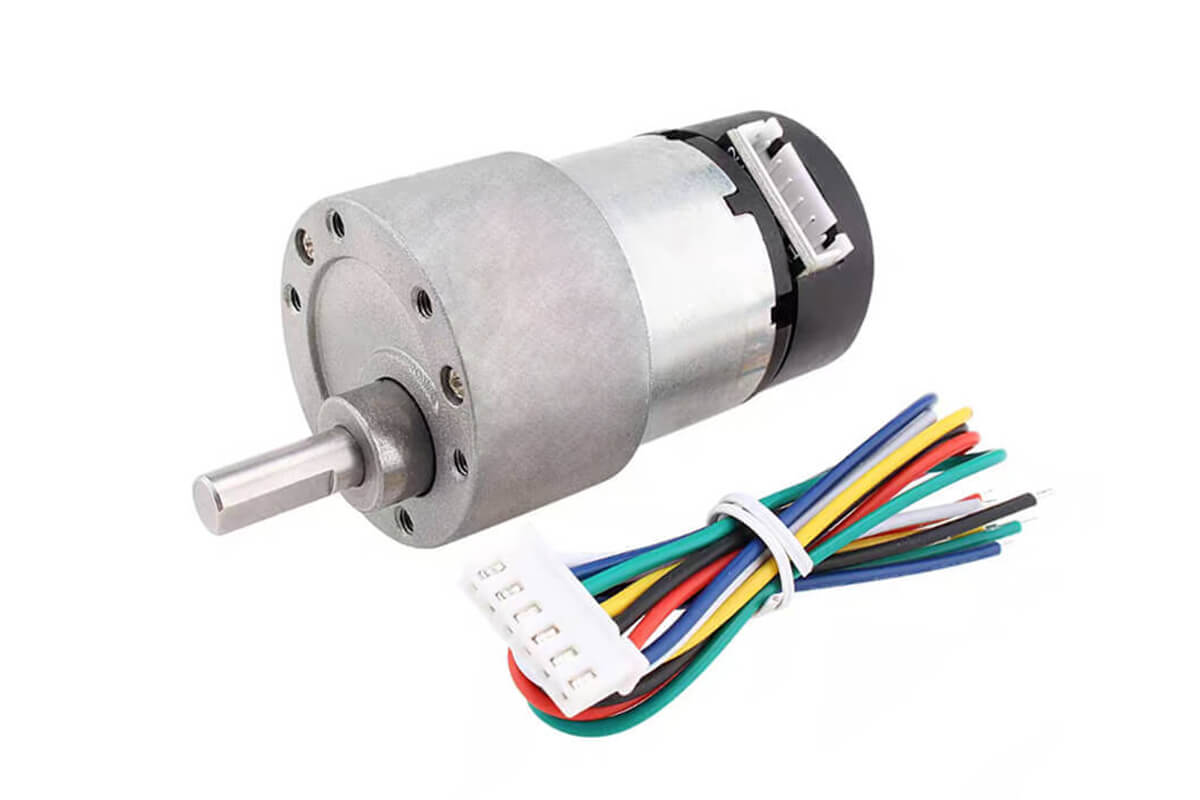
\includegraphics[height=4cm]{assets/dc-motor-with-encoder.jpg}
	\caption{Similar construction motors were used in this project \cite{dc_motor}.}
	\label{fig:dc-motor}
\end{figure}

\subsection{Hierarchical Control Strategy}
To optimize system performance and resource utilization, the control loop employs a hierarchical update strategy:
\begin{itemize}
	\item \textbf{Pitch Control}: Updated at the highest frequency (e.g., every control cycle) to ensure rapid response to changes in the robot's tilt and maintain balance.
	\item \textbf{Yaw and Position Control}: Updated at a lower frequency (e.g., every 8th cycle) to reduce computational load while still providing adequate motion control.
\end{itemize}

This approach prioritizes critical tasks (e.g., maintaining balance) while efficiently managing system resources, ensuring robust and stable operation.


\subsection{Basic PID Structure}
The PID controller generates a control signal $u(t)$ based on the error signal $e(t)$, which is the difference between the desired setpoint and the measured process variable (see Fig. \ref{fig:control-loop-block-diagram}). The control signal is computed as:

\begin{equation}
	u(t) = K_p e(t) + K_i \int_0^t e(\tau)d\tau + K_d \frac{d}{dt}e(t)
\end{equation}

Where:
\begin{itemize}
	\item $u(t)$: Control signal applied to the system.
	\item $e(t)$: Error signal, representing the deviation from the setpoint.
	\item $K_p$: Proportional gain, which responds to the current error.
	\item $K_i$: Integral gain, which addresses accumulated past errors.
	\item $K_d$: Derivative gain, which predicts future error trends based on the rate of change.
\end{itemize}

\subsection{Discrete Time Implementation}
For digital implementation, the continuous-time PID equation is discretized to suit microcontroller-based systems. The discrete-time PID control signal u[n]u[n] is calculated as:

\begin{equation}
	u[n] = K_p e[n] + K_i T_s \sum_{k=0}^n e[k] + K_d \frac{e[n] - e[n-1]}{T_s}
\end{equation}

where:
\begin{itemize}
 \item $T_s$: Sampling period, representing the time interval between consecutive control updates.
 \item $e[n]$: Error signal at the nn-th sampling instant.
 \item $u[n]$: Control signal at the nn-th sampling instant.
\end{itemize}
This formulation ensures compatibility with real-time embedded systems while maintaining control precision.


\subsubsection{Power Supply considerations}
The custom-designed battery box (shown in Fig.~\ref{fig:battery}) provides a portable and rechargeable power solution for the Elegoo robot~\cite{battery}. It houses two 18650 LiPo batteries, likely connected in series, to deliver a regulated voltage suitable for powering the robot’s components. An integrated Battery Management System (BMS) ensures safe operation by protecting against overcharge, over-discharge, over-current, and short circuits. A power switch enables complete disconnection, while a USB charging port and status indicator LED facilitate easy recharging and monitoring.  

\begin{figure}[h]
	\centering
	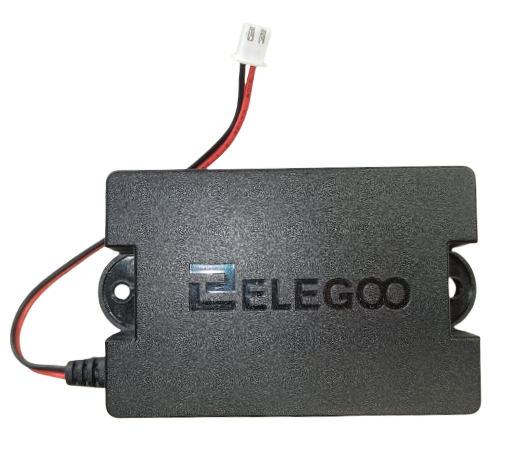
\includegraphics[height=6cm]{assets/Battery.png}
	\caption{ELEGOO battery pack with charger.}
	\label{fig:battery}
\end{figure}

To monitor battery voltage, the Arduino Nano employs a voltage divider circuit, scaling the battery voltage to a safe range for its analog-to-digital converter (ADC). The divider consists of two resistors in series, and the output voltage is given by:  
\begin{equation}  
	V_{\text{out}} = V_{\text{battery}} \times \frac{R_2}{R_1 + R_2}  
\end{equation}  

where \( V_{\text{out}} \) is the scaled-down voltage read by the Arduino’s ADC, and \( R_1 \) and \( R_2 \) are the resistor values chosen to ensure the measured voltage remains within the 0–5V range.  

\begin{figure}[H]  
	\centering  
	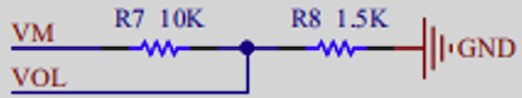
\includegraphics[height=1cm]{assets/voltage-divider.png}  
	\caption{Voltage divider circuit used for in the robot \cite{tumbller}.}  
	\label{fig:voltage-divider}  
\end{figure}

The A2 pin is used for measurement, and the internal reference voltage is set to 1.1V, ensuring stable readings independent of supply voltage fluctuations. However, since 1.1V is too low to directly measure the battery voltage, a resistor divider is implemented. A 10k\(\Omega\) (R1) and 1.5k\(\Omega\) (R2) resistor pair (schematic shown in Fig.~\ref{fig:schematics_control-loop}) is used, forming a 1/11 voltage division ratio:
\begin{equation}  
	V_{\text{out}} = V_{\text{battery}} \times \frac{1.5}{10 + 1.5} = V_{\text{battery}} \times 0.136  
\end{equation}  

For a fully charged 8.4V LiPo battery, the resulting $ V_{\text{out}} \approx $ 1.14 V, which is safely within the 1.1 V reference range but may introduce minor ADC saturation at peak voltage.

The following function reads the battery voltage using the voltage divider and determines the battery status:
\begin{lstlisting}[style=cppstyle2]
void Voltage_Measure()
{
	if (millis() - vol_measure_time > 1000) //Measured every 1000 milliseconds
	{
		vol_measure_time = millis();
		double voltage = (analogRead(VOL_MEASURE_PIN) * 1.1 / 1024) * ((10 + 1.5) / 1.5); //Read voltage value
		Serial.print("Current voltage value : ");
		Serial.println(voltage);
		if(voltage>7.8)
		Serial.println("The battery is fully charged");
		else
		Serial.println("Low battery");
	}
}
\end{lstlisting}


\subsection{Tuning Methodology}
The Ziegler-Nichols method is a widely used and systematic approach for tuning PID controllers. It provides a reliable framework for determining initial controller parameters, which can then be fine-tuned for optimal performance. The method involves inducing controlled oscillations in the system to identify critical parameters, which are then used to calculate the proportional, integral, and derivative gains.
\subsubsection{Ziegler-Nichols Method}
The Ziegler-Nichols tuning procedure consists of the following steps:
\begin{enumerate}
	\item \textbf{Initialize Parameters}: Set the integral gain \( K_i \) and derivative gain \( K_d \)to zero, leaving only the proportional gain \( K_p \) active.
	\item \textbf{Induce Oscillations}: Gradually increase \( K_p \) until the system exhibits sustained oscillations. At this point, the system is at the threshold of stability, and the proportional gain is referred to as the ultimate gain \( K_u \). The period of these oscillations is denoted as \( T_u \).
	\item \textbf{Record Critical Values}: Note the values of \( K_u \) and \( T_u \), as they are essential for calculating the final PID parameters.
	\item \textbf{Calculate PID Gains:} Using the recorded values, compute the PID parameters as follows:
	\begin{equation}
	\begin{aligned}
		K_p &= 0.6K_u \\
		T_i &= 0.5T_u \\
		T_d &= 0.125T_u  \label{eq:eq}
	\end{aligned}
	\end{equation}
	Here, \( T_i \) and \( T_d \) represent the integral and derivative time constants, respectively. These values are then used to determine the integral and derivative gains:
	\begin{equation}
	\begin{aligned}
	K_i = \frac{K_p}{T_i} \quad \text{and} \quad K_d = K_p \cdot T_d.  \label{eq:eq}
	\end{aligned}
	\end{equation}
\end{enumerate}
	
This method provides a robust starting point for achieving stable control. However, it is important to note that the Ziegler-Nichols method may require additional fine-tuning to account for system-specific dynamics and performance requirements. The calculated parameters serve as an initial baseline, which can be further optimized through iterative testing and adjustment.


\subsubsection{Practical Tuning Guidelines}
In addition to the Ziegler-Nichols method, practical tuning guidelines were applied to refine the controller performance:

\begin{itemize}
	\item Start with a small proportional gain $K_p$ (e.g. $K_p$ = 10) to avoid instability.
	\item Introduce the derivative term $K_d$ to dampen oscillations, typically setting $K_d = 0.1K_p$.
	\item  Fine-tune $K_p$, $K_i$, and $K_d$ iteratively to achieve optimal stability and responsiveness.
\end{itemize}


\subsection{Pitch PID Control:}
The pitch control loop ensures the robot maintains its upright position. The primary objective of the pitch controller is to minimize the deviation of the robot's pitch angle from a set-point, which is ideally zero degrees (i.e., upright). The pitch control output is calculated using the PD algorithm, where the error is the difference between the current pitch angle and the desired pitch angle. 
\begin{equation}
	\tau_{\theta,pid} = K_{p\theta}({\theta_{desired} - \theta_{measured}}) + K_{d\theta}\frac{d}{dt}(\theta_{desired} - \theta_{measured})
\end{equation}

Below is its code implementation:
\begin{lstlisting}[style=cppstyle2]
inline void runPitchControl() {
	pitch_pid_output = (kp_balance * (kalman.angle - 0)) + (kd_balance * gyro_x);
}
\end{lstlisting}

The final results are shown in Fig.~\ref{fig:pid_position_kp_55_kd_1_25}.
\begin{figure}[H]
	\centering
	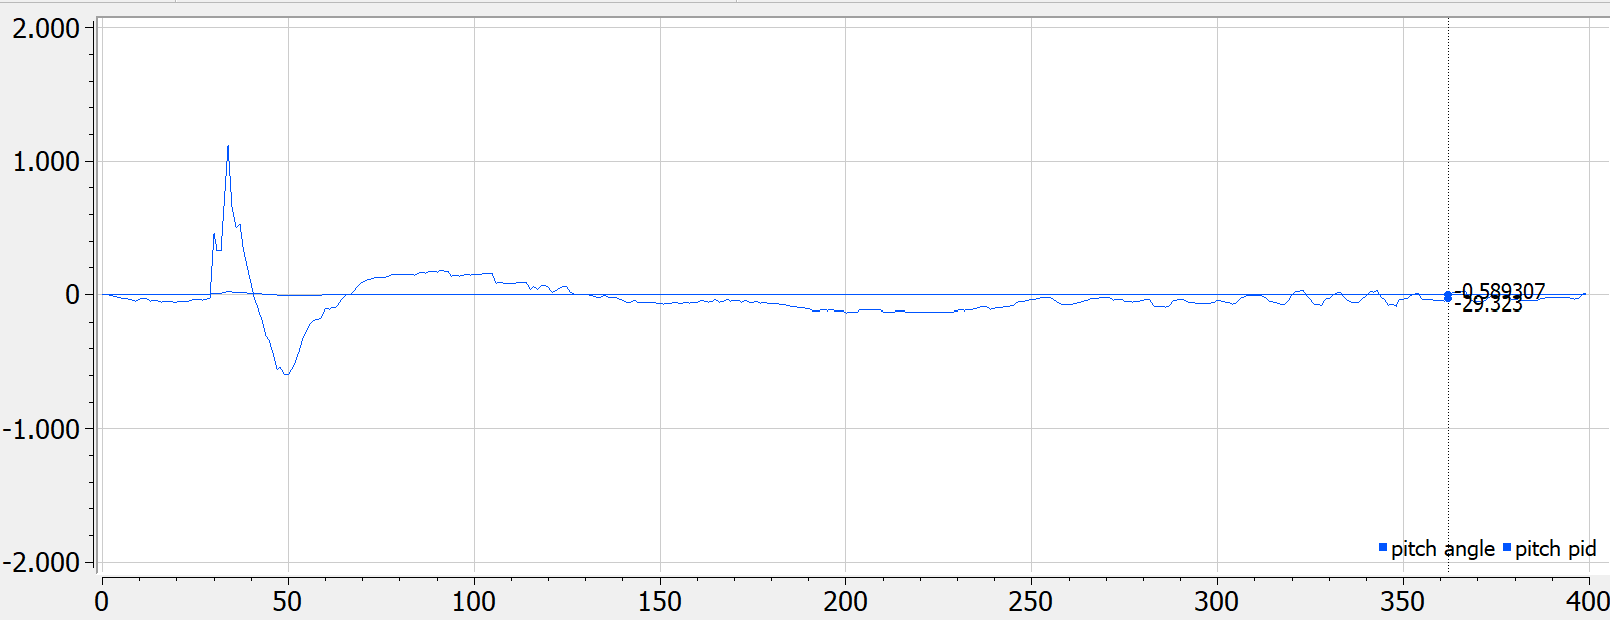
\includegraphics[width=0.8\linewidth]{assets/pid_pitch_kp_55_kd_1_25.png}
	\caption{Pitch angle control system response at $K_{p\theta}$ = 55 and $K_{d\theta}$ = 1.25. The data was recorded at baud rate of 115200.}
	\label{fig:pid_position_kp_55_kd_1_25}
\end{figure}

\subsection{Eliminating Jitter}
Once the system reaches stability, it begins to exhibit jitter, as observed in the PID output between data points 250 and 400 in Fig.~\ref{fig:pid_position_kp_55_kd_1_25}. This jitter arises due to the high sensitivity of the derivative gain ($K_{d\theta}$) to fluctuations in the gyroscope readings ($\dot{\theta}$). While reducing $K_{d\theta}$ mitigates the jitter, it also diminishes the system's ability to dampen oscillations, leading to excessive overshoot and potential instability. Fig.~\ref{fig:pid_position_overshoot} illustrates the system's response when using $K_{p\theta}$ = 55 and $K_{d\theta}$ = 0.75 where significant overshoot is evident.

\begin{figure}[H]
	\centering
	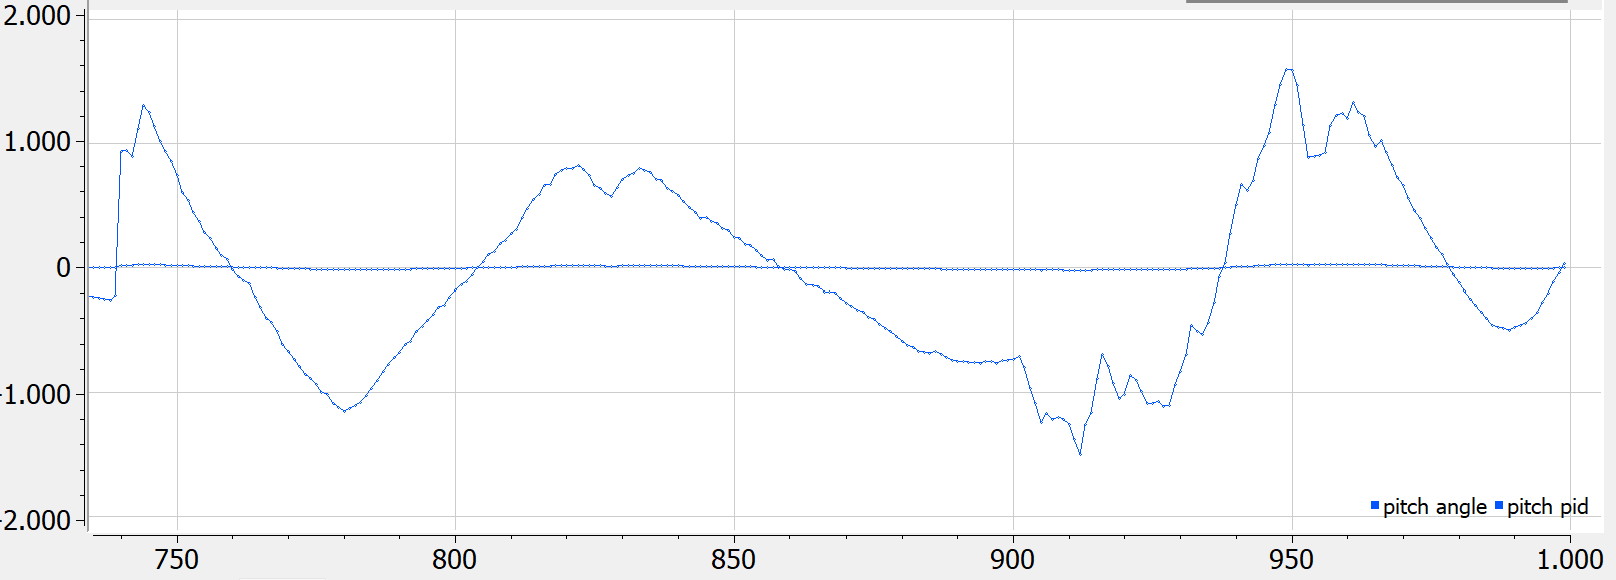
\includegraphics[width=0.8\linewidth]{assets/pid_pitch_overshoot.png}
	\caption{Pitch angle control system response at $K_{p\theta}$ = 55 and $K_{d\theta}$ = 0.75. Data recorded at baud rate of 115200.}
	\label{fig:pid_position_overshoot}
\end{figure}

To address this issue, an \textbf{adaptive derivative gain approach} is implemented, where $K_{d\theta}$ is adjusted dynamically based on the pitch angle of the robot. When the absolute pitch angle exceeds a predefined threshold, a higher derivative gain is used to provide stronger correction, while a lower gain is applied for small angles to minimize jitter. The corresponding implementation is as follows:
\begin{lstlisting}[style=cppstyle2]
if (pitch_angle > 8) { kd_balance = kd_balance_large_angle; }
else { kd_balance = kd_balance_small_angle; }

inline void runPitchControl() {
	pitch_pid_output = (kp_balance * (kalman.angle - 0)) + (kd_balance * gyro_x);
}
\end{lstlisting}

This adaptive control strategy effectively stabilizes the system while reducing excessive oscillations. Fig.~\ref{fig:pid_position_combined} presents the improved system response, demonstrating a smoother transition and enhanced overall stability.
\begin{figure}[H]
	\centering
	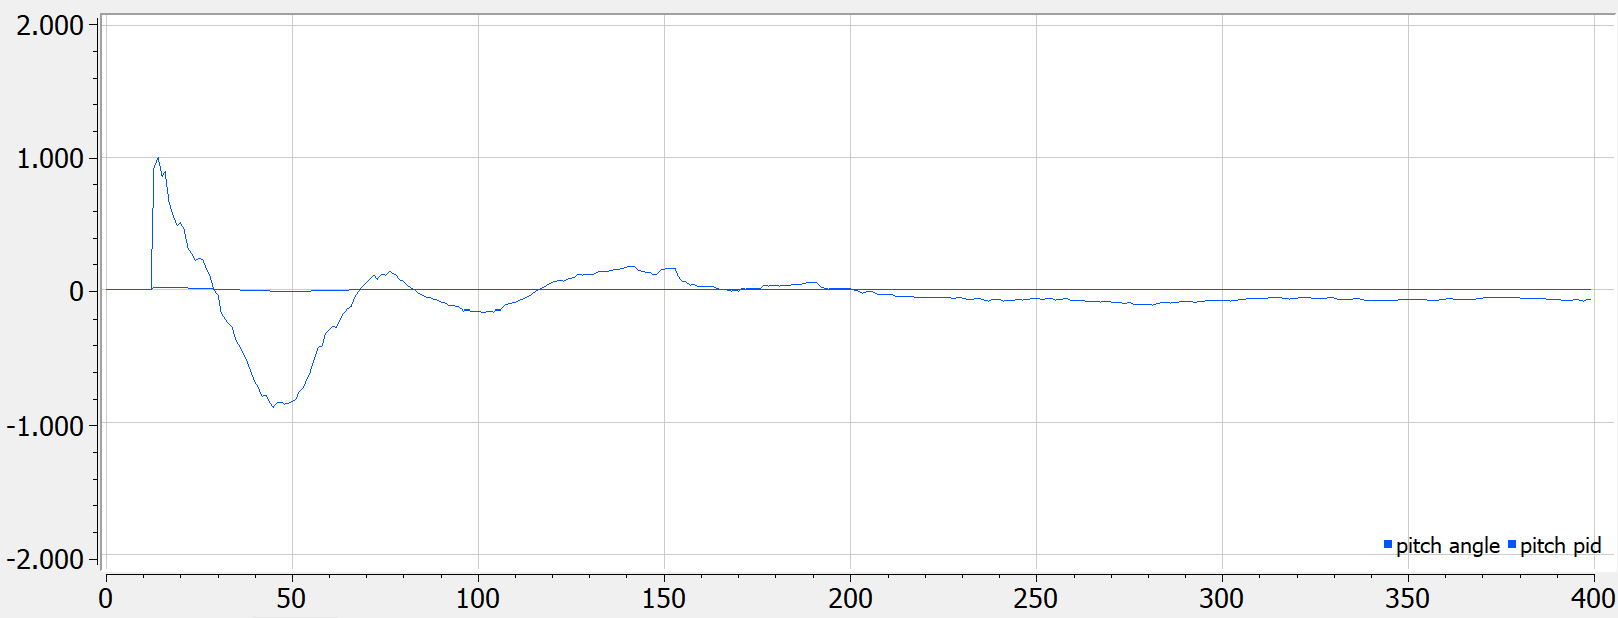
\includegraphics[width=0.8\linewidth]{assets/pid_pitch_combined.png}
	\caption{Pitch angle control system response. The data was recorded at baud rate of 115200.}
	\label{fig:pid_position_combined}
\end{figure}


\subsection{Yaw Control:}
Yaw control is responsible for controlling the robot's rotational movement around its vertical axis. The yaw PID controller computes the control output based on the robot's angular velocity, which is measured by the gyroscope along the z-axis. 
\begin{equation}
	\tau_{\phi,pid} = K_{p\phi}(\phi_{desired} - \phi_{measured}) + K_{d\phi}\frac{d}{dt}(\phi_{desired} - \phi_{measured})
\end{equation}

Below is its code implementation:
\begin{lstlisting}[style=cppstyle2]
inline void runYawControl(){
	float delta_yaw_angle = yaw_angle_degrees - desired_yaw_angle;
	yaw_pid_output = (kp_turn * delta_yaw_angle) + (kd_turn * gyro_z);
}
\end{lstlisting}

The yaw control adjusts the motor speeds to achieve the desired angle, ensuring the robot maintains a stable heading. Fig.~\ref{fig:pid_yaw} illustrates the system's response with \(K_{p\phi}\) = 2.5 and $K_{i\phi}$ = 0.5 when transitioning from an initial angle of $-20 \ deg$ to final angle of $+20 \ deg$.
\begin{figure}[H]
	\centering
	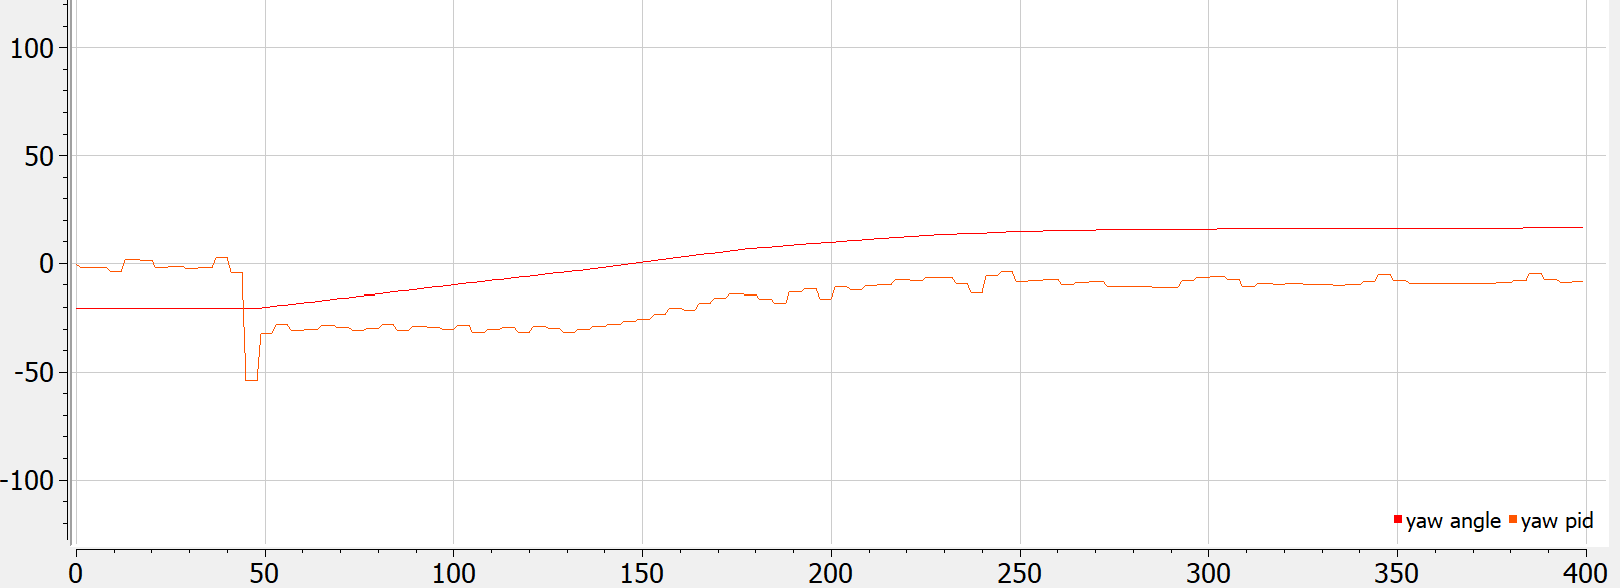
\includegraphics[width=0.8\linewidth]{assets/pid_yaw_kp_2_5_kd_0_5_target_20_deg.png}
	\caption{Yaw angle control system response at \(K_p\) = 2.5 and $K_i$ = 0.5 for an angle transition from $-20 \ deg$ to $+20 \ deg$. The data was recorded at baud rate of 115200.}
	\label{fig:pid_yaw}
\end{figure}

\subsection{Position Control:}
Position control is implemented to ensure the robot moves smoothly and accurately along a path or to a target location. The encoder feedback from the left and right wheels is used to calculate the robot's displacement and speed. The position PID controller adjusts the motor speeds to minimize the error in position and velocity.
\begin{equation}
	\tau_{x,pid} = K_{px}(x_{desired} - x_{measured}) + K_{dx}\frac{d}{dt}(x_{desired} - x_{measured})
\end{equation}

Below is its code implementation:
\begin{lstlisting}[style=cppstyle2]
inline void runPositionControl(){
	position_pid_output = - (kp_position * (current_position - move_to_position)) - (kd_position * encoder_speed_filtered);
}
\end{lstlisting}

The position controller continuously adjusts motor speeds to reduce position error while maintaining a stable heading. Fig.~\ref{fig:pid_postition} presents the system's response when \(K_{px}\) = 0.26 and $K_{dx}$ = 20 when moving from relative distance of $-20 \ cm$ to $+20 \ cm$.
\begin{figure}[H]
	\centering
	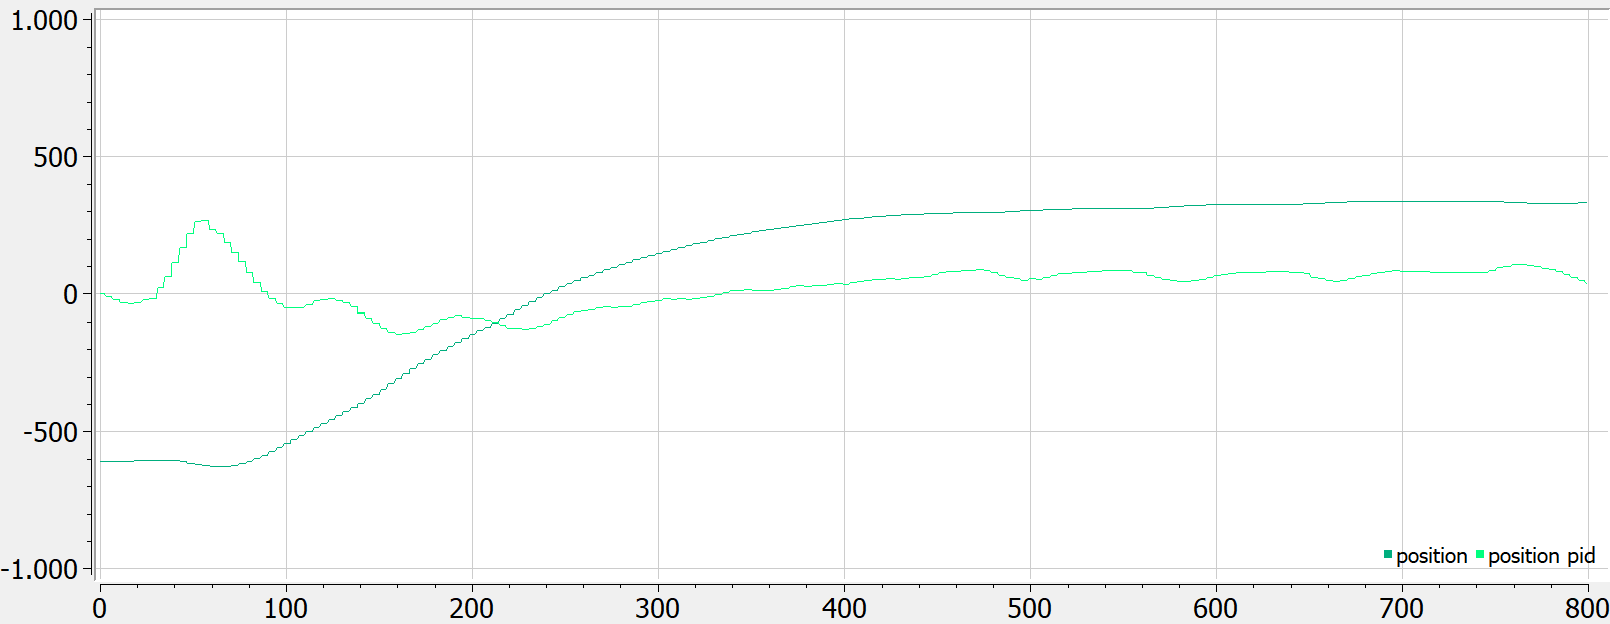
\includegraphics[width=0.8\linewidth]{assets/pid_position_kp_0_26_kd_20.png}
	\caption{Position control system response with \(K_{px}\) = 0.26 and $K_{dx}$ = 20 for a displacement of $-20 \ cm$ to $+20 \ cm$. Data recorded at baud rate of 115200.}
	\label{fig:pid_postition}
\end{figure}


\subsection{Combining Control Outputs}
The final motor control is achieved by combining the outputs from all three PID controllers. The outputs from the pitch, yaw, and position PID controllers are used to calculate the motor speeds, which determine the robot's motion. Specifically, the following equation is used to compute the PWM values for the left and right motors:

\begin{align}
	\tau_{left,motor} &= \tau_{\theta,pid} - \tau_{\phi,pid} - \tau_{x,pid} \\
	\tau_{right,motor} &= \tau_{\theta,pid} + \tau_{\phi,pid} - \tau_{x,pid}
\end{align}

Below is its code implementation:
\begin{lstlisting}[style=cppstyle2]
void balance(){
...
			
	pwm_left = pitch_pid_output - yaw_pid_output - position_pid_output;
	pwm_right = pitch_pid_output + yaw_pid_output - position_pid_output;

...
}
\end{lstlisting}

The computed Pulse-Width-Modulation (PWM) are transmitted to the motor drivers, which adjust the robot's movement and balance in real time. This closed-loop control mechanism ensures precise and stable operation by continuously refining motor outputs based on sensor feedback. A simplified diagram of the motor control loop is illustrated in Fig.~\ref{fig:schematics_control-loop}.

\begin{figure}[H]
	\centering
	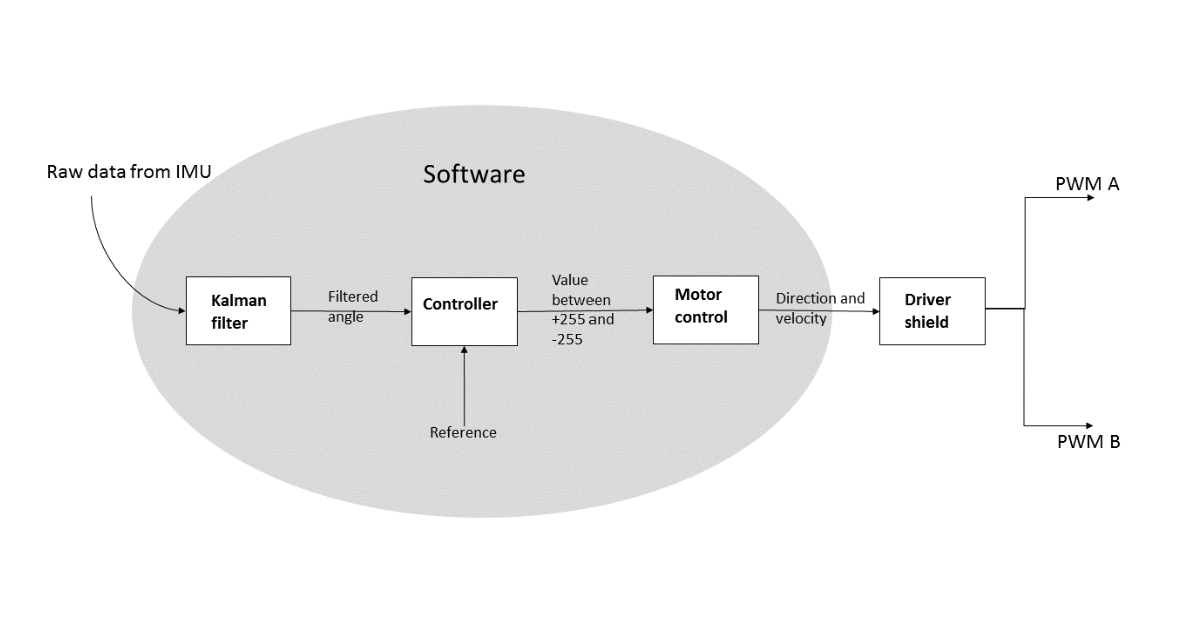
\includegraphics[height=8cm]{assets/pitch_angle_control_loop.png}
	\caption{A simplified diagram of the motor control loop \cite{10193276}.}
	\label{fig:schematics_control-loop}
\end{figure}


\subsection{Results}
The use of PID controllers for pitch, yaw, and position control enables the robot to maintain balance and navigate effectively (see Fig. \ref{fig:control-loop-2}). The proportional, integral, and derivative terms in each PID loop allow the system to respond to real-time errors, minimize steady-state deviations, and anticipate future errors, leading to smooth and precise control of the robot's motion. The integration of these PID controllers is fundamental to the robot's stability and performance. Final results are shown in Fig.~\ref{fig:final_pid}

\begin{figure}[h]
	\centering
	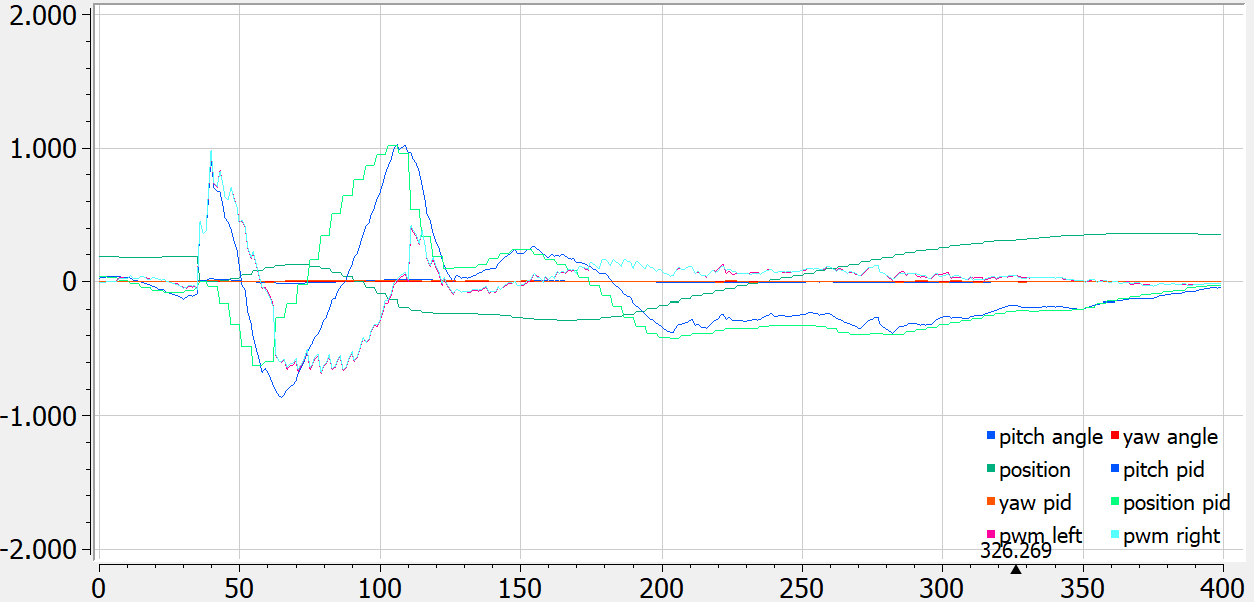
\includegraphics[width=0.8\linewidth]{assets/final_pid.png}
	\caption{The final control system individual output values recorded at baud rate of 115200.}
	\label{fig:final_pid}
\end{figure}

\begin{figure}[h]
	\centering
	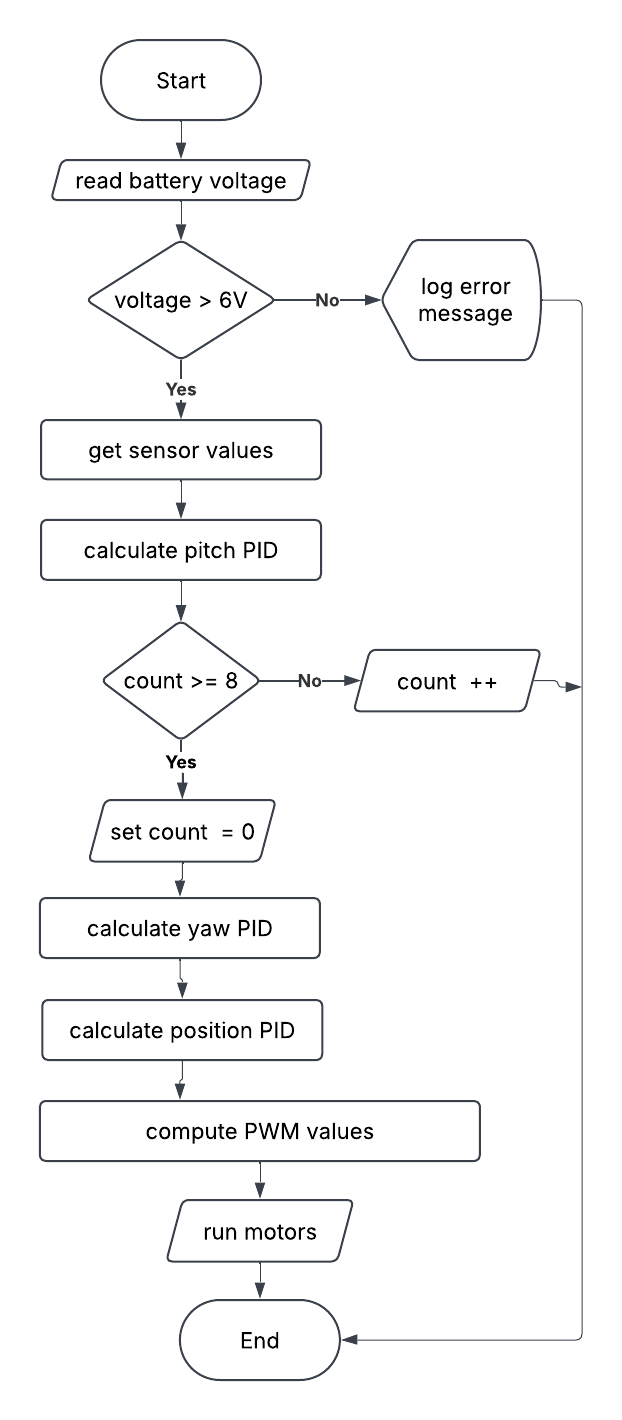
\includegraphics[width=0.5\linewidth]{assets/control_loop_diagram.png}
	\caption{A simplified block diagram of the cascaded control loop used. }
	\label{fig:control-loop-2}
\end{figure}

	
\subsection{Front Obstacle Detection}
The Ultrasonic distance measuring sensor is used to detect the obstacle in front of the robot.

\subsection{Ultrasonic Working Principle}
The sensor consists of a \textbf{transmitter} and a \textbf{receiver}:
\begin{itemize}
	\item The transmitter emits an ultrasonic pulse (40 kHz).
	\item The pulse reflects off an obstacle and is received by the receiver.
	\item The time difference between transmission and reception is used to compute the distance using the formula:
\end{itemize}
\begin{equation}
	d = \frac{t \times v}{2}
\end{equation}
where:
\begin{itemize}
	\item \(d\) is the measured distance,
	\item \(t\) is the time delay (in microseconds),
	\item \(v\) is the speed of sound (approximately 343 m/s at room temperature).
\end{itemize}

\subsubsection{Ultrasonic Implementation}
The HC-SR04 requires control signals to be sent from a microcontroller:
\begin{enumerate}
	\item A short \textbf{trigger pulse} is sent to the \texttt{TRIG} pin.
	\item The sensor responds with a high signal on the \texttt{ECHO} pin.
	\item The duration of the \texttt{ECHO} signal is measured to determine the distance.
\end{enumerate}

\subsubsection{Code for Distance Measurement}Based on the datasheet \cite{ultra-sonic}, an operating frequency of 20 Hz (corresponding to a 50 ms interval) is selected for distance measurements. The speed of sound is taken as 340.29 m/s, leading to the following constants in the code:

\begin{lstlisting}[style=cppstyle2]
	constexpr uint8_t USONIC_GET_DISTANCE_DELAY_MS = 50;
	constexpr float SPEED_OF_SOUND_HALVED = (340.29 * 100.0) / (2 * 1000 * 1000);
\end{lstlisting}

Here, the speed of sound is converted to cm/µs, and it is divided by 2 to account for the round-trip travel time of the ultrasonic pulse. The following C++ function is used to initiate distance measurement using the HC-SR04 ultrasonic sensor:
\begin{lstlisting}[style=cppstyle2]
void StartUltrasonicMeasurement() {
	if (millis() - usonicGetDistancePrevTime > USONIC_GET_DISTANCE_DELAY_MS) {
		usonicMeasureFlag = SEND;
		usonicGetDistancePrevTime = millis();
		
		attachPinChangeInterrupt(ECHO_PIN, HandleUltrasonicMeasurementInterrupt, RISING);
		
		digitalWrite(TRIG_PIN, LOW);
		digitalWrite(TRIG_PIN, HIGH);
		digitalWrite(TRIG_PIN, LOW);
	}
\end{lstlisting}

\begin{itemize}
	\item The function \texttt{StartUltrasonicMeasurement()} ensures that the measurement is taken at regular intervals.
	\item A global flag \texttt{usonicMeasureFlag} is set to \texttt{SEND}, indicating that the trigger pulse is sent.
	\item The function \texttt{attachPinChangeInterrupt()} attaches an interrupt to detect when the \texttt{ECHO} pin goes HIGH.
	\item The \texttt{TRIG} pin is first set LOW (to reset), then HIGH (to trigger the pulse), and then set LOW again.
\end{itemize}
This setup enables precise distance measurement by capturing the time delay between sending and receiving the ultrasonic pulse.


\subsubsection{Interrupt Service Routine}
The following function handles the interrupt to measure the distance:

\begin{lstlisting}[style=cppstyle2]
	void HandleUltrasonicMeasurementInterrupt() {
		if (usonicMeasureFlag == SEND) {
			usonicMeasurePrevTime = micros();
			attachPinChangeInterrupt(ECHO_PIN, HandleUltrasonicMeasurementInterrupt, FALLING);
			usonicMeasureFlag = RECEIVED;
		} else if (usonicMeasureFlag == RECEIVED) {
			usonicDistanceValue = (uint8_t)((micros() - usonicMeasurePrevTime) * SPEED_OF_SOUND_HALVED);
			usonicMeasureFlag = IDLE;
		}
	}
\end{lstlisting}

\begin{itemize}
	\item When the echo signal first rises (RISING edge), the timestamp is recorded using \texttt{micros()}.
	\item The interrupt is then reattached to detect the falling edge.
	\item When the falling edge is detected, the elapsed time is computed.
	\item The time is converted to distance using the speed of sound formula.
	\item Finally, the system resets for the next measurement.
\end{itemize}


\subsubsection{Infrared Sensing Implementation}
The IR LED transmits a modulated 38kHz infrared signal. If an obstacle is present, the signal reflects and is received by the IRM-56384, which demodulates the signal and provides a digital output. The following code is used to control and process the IR proximity sensors:
\begin{lstlisting}[style=cppstyle2]
	void IRSesorSend38KPule(unsigned char ir_pin){
		for( int i = 0; i < 39; i++) {
			digitalWrite(ir_pin, LOW);
			delayMicroseconds(9);
			digitalWrite(ir_pin, HIGH);
			delayMicroseconds(9);
		}
	}
	
	void ProcessLeftIRSensor(){
		if (millis() - irLeftCountTime > IR_COUNT_DELAY_MS) {
			UpdateSlidingWindow(irLeftPulseCount >= 3, irLeftHistory, irLeftIndex, irLeftRunningCount);    
			irLeftIsObstacle = (irLeftRunningCount >= 5);
			irLeftPulseCount = 0;
			irLeftCountTime = millis();
		}
	}
	
	void ProcessRightIRSensor(){
		if (millis() - irRightCountTime > IR_COUNT_DELAY_MS) {
			UpdateSlidingWindow((irRightPulseCount >= 3), irRightHistory, irRightIndex, irRightRunningCount);
			irRightIsObstacle = (irRightRunningCount >= 5);
			irRightPulseCount = 0;
			irRightCountTime = millis();
		}
	}
\end{lstlisting}

	\section{Remote Control and Communication}

The remote control and communication system of the two-wheeled self-balancing robot was designed to enable seamless and reliable interaction between the user and the robot. For this purpose, we integrated the \textbf{BT16 Bluetooth UART Module}, which provided a robust wireless communication link.

\subsection{Bluetooth Module Integration}
The \textbf{BT16 Bluetooth UART Module} was chosen due to its compatibility with microcontrollers and its ability to provide stable serial communication over Bluetooth. The module was interfaced with the microcontroller using UART communication, ensuring efficient data transmission and reception.

\subsection{Communication Protocol}
A custom communication protocol was developed to manage the exchange of control commands and telemetry data. Key features of the protocol included:

\begin{itemize}
\item \textbf{Command Transmission:} The robot could receive commands for movement control, mode switching, and parameter adjustments from a remote device.
\item \textbf{Telemetry Feedback:} The robot transmitted real-time data such as tilt angle, battery status, and motor performance back to the controlling device.
\item \textbf{Error Handling:} Mechanisms were implemented to detect and recover from communication errors, ensuring reliable operation even in noisy environments.
\end{itemize}

\subsection{User Interface for Remote Control}
The Bluetooth communication enabled the development of a user-friendly interface for remote control. This interface could be a mobile application or a desktop-based GUI, allowing users to interact with the robot intuitively. Features included:

\begin{itemize}
\item \textbf{Joystick Control:} For real-time maneuvering of the robot.
\item \textbf{Status Monitoring:} Display of critical telemetry data.
\item \textbf{Parameter Tuning:} On-the-fly adjustment of control parameters for performance optimization.
\end{itemize}

\subsection{Testing and Performance}
Extensive testing was conducted to ensure the reliability and responsiveness of the Bluetooth communication system. The tests focused on:

\begin{itemize}
\item \textbf{Range:} Assessing the effective communication distance.
\item \textbf{Latency:} Measuring the delay between command transmission and robot response.
\item \textbf{Stability:} Ensuring consistent performance in various environments.
\end{itemize}

The integration of the Bluetooth module significantly enhanced the robot's usability, providing a flexible and responsive remote control solution that contributed to the overall functionality and user experience of the system.
	%\section{Simulation and Testing}
Simulation and testing played a crucial role in the development and refinement of the two-wheeled self-balancing robot. By leveraging computational tools and environments, we were able to model the robot's behavior under various conditions, validate control algorithms, and predict system performance before real-world implementation.

\subsection{Simulation Tools and Environment}
For simulating the dynamics and control strategies of the robot, we utilized both \textbf{Python} and \textbf{MATLAB}. These platforms provided robust frameworks for numerical computation, visualization, and algorithm development.

\begin{itemize}
\item \textbf{Python:} Utilized libraries such as \textit{NumPy}, \textit{SciPy}, and \textit{Matplotlib} for numerical simulations and visualizations. \textit{Control} and \textit{SymPy} libraries were used to model the control systems and analyze the system's response.
\item \textbf{MATLAB:} Employed for more advanced control design and simulation, including the use of Simulink for block diagram modeling and simulation of dynamic systems. MATLAB's built-in tools facilitated the tuning and optimization of control parameters.
\end{itemize}

\subsection{Control Algorithm Testing}
We implemented and tested various control algorithms to ensure the stability and performance of the robot. Key focus was given to the \textbf{Complementary Filter} and \textbf{Kalman Filter} for sensor fusion and state estimation.

\begin{itemize}
\item \textbf{Complementary Filter:} Simulations helped fine-tune the filter coefficients to effectively merge accelerometer and gyroscope data, providing a stable estimate of the robot's tilt angle.
\item \textbf{Kalman Filter:} The filter was tested for its ability to reduce noise and provide accurate state estimation. MATLAB simulations were crucial in visualizing the filter's performance and adjusting the covariance matrices.
\end{itemize}

\subsection{Performance Metrics}
Several metrics were used to evaluate the performance of the control algorithms in the simulation environment:

\begin{itemize}
\item \textbf{Stability:} Assessed by analyzing the system's ability to return to an upright position after disturbances.
\item \textbf{Response Time:} Measured how quickly the control system could react to changes in tilt and external perturbations.
\item \textbf{Noise Rejection:} Evaluated the effectiveness of the filters in minimizing sensor noise and maintaining accurate state estimation.
\end{itemize}

\subsection{Real-World Validation}
Post-simulation, the control algorithms were transferred to the physical robot for real-world testing. The outcomes from the simulations provided a strong baseline, and discrepancies observed during physical trials were fed back into the simulation models for further refinement. This iterative process ensured a robust and reliable control system.

Overall, the combination of Python and MATLAB simulations significantly accelerated the development process and provided valuable insights into the robot's dynamic behavior and control performance.

\section{Simulation and Testing}

Simulation and testing played a crucial role in the development and refinement of the two-wheeled self-balancing robot. By leveraging computational tools and environments, we were able to model the robot's behavior under various conditions, validate control algorithms, and predict system performance before real-world implementation.

\subsection{Simulation Tools and Environment}
For simulating the dynamics and control strategies of the robot, we utilized both \textbf{Python} and \textbf{MATLAB}. These platforms provided robust frameworks for numerical computation, visualization, and algorithm development.

\subsection{PID Tuning}
\subsubsection{}
\subsubsection{PID Tuning Results}
Response specifications No Load With Loads 
Initial Deviation 
Rise Time
Peak Time
Maximum Overshoot
Settling Time
Error Steady State

\begin{itemize}
\item \textbf{Python:} Utilized libraries such as \textit{NumPy}, \textit{SciPy}, and \textit{Matplotlib} for numerical simulations and visualizations. \textit{Control} and \textit{SymPy} libraries were used to model the control systems and analyze the system's response.
\item \textbf{MATLAB:} Employed for more advanced control design and simulation, including the use of Simulink for block diagram modeling and simulation of dynamic systems. MATLAB's built-in tools facilitated the tuning and optimization of control parameters.
\end{itemize}

\subsection{Control Algorithm Testing}
We implemented and tested various control algorithms to ensure the stability and performance of the robot. Key focus was given to the \textbf{Complementary Filter} and \textbf{Kalman Filter} for sensor fusion and state estimation.

\begin{itemize}
\item \textbf{Complementary Filter:} Simulations helped fine-tune the filter coefficients to effectively merge accelerometer and gyroscope data, providing a stable estimate of the robot's tilt angle.
\item \textbf{Kalman Filter:} The filter was tested for its ability to reduce noise and provide accurate state estimation. MATLAB simulations were crucial in visualizing the filter's performance and adjusting the covariance matrices.
\end{itemize}

\subsection{Performance Metrics}
Several metrics were used to evaluate the performance of the control algorithms in the simulation environment:

\begin{itemize}
\item \textbf{Stability:} Assessed by analyzing the system's ability to return to an upright position after disturbances.
\item \textbf{Response Time:} Measured how quickly the control system could react to changes in tilt and external perturbations.
\item \textbf{Noise Rejection:} Evaluated the effectiveness of the filters in minimizing sensor noise and maintaining accurate state estimation.
\end{itemize}

\subsection{Real-World Validation}
Post-simulation, the control algorithms were transferred to the physical robot for real-world testing. The outcomes from the simulations provided a strong baseline, and discrepancies observed during physical trials were fed back into the simulation models for further refinement. This iterative process ensured a robust and reliable control system.


To thoroughly test the robustness of the system, we introduced controlled disturbances and varying surface conditions in the real-world environment. This helped identify edge cases and stress points that were not evident in the simulation phase. By iteratively refining the control algorithms based on these findings, we were able to enhance the overall stability and performance of the robot.

Overall, the combination of Python and MATLAB simulations significantly accelerated the development process and provided valuable insights into the robot's dynamic behavior and control performance.


	%\section{Power Management}

Efficient power management was critical for ensuring the longevity and reliability of the two-wheeled self-balancing robot. We employed \textbf{7.4V Lithium-Ion battery packs} to provide a stable power supply.

\subsection{Battery Selection and Integration}
The 7.4V Lithium-Ion battery packs were chosen for their high energy density, lightweight properties, and reliable performance. These batteries were integrated with a voltage regulator circuit to ensure consistent voltage levels to the microcontroller and motor drivers.

\subsection{Power Monitoring}
To monitor the battery status in real-time, voltage sensors were used to track battery levels. This data was integrated into the telemetry feedback system, allowing the user to receive alerts when the battery level was low.

\subsection{Charging and Safety}
A dedicated charging circuit with overcharge protection was implemented to enhance battery life and safety. Thermal sensors were also included to monitor battery temperature during operation and charging.
	%\section{User Interface}
The user interface (UI) for the robot is designed to facilitate interactive control and real-time monitoring. It integrates command parsing, telemetry data handling, and communication protocols such as Inter-Integrated Circuit (I2C) and Universal Asynchronous Receiver-Transmitter (UART). Users can send commands to the robot and receive real-time telemetry feedback, ensuring efficient control and monitoring.

Communication is structured around well-defined command and telemetry packets, implemented in \texttt{comm.hpp}. These packets support multiple data formats, ensuring compatibility with various communication protocols. The functions responsible for sending and receiving telemetry data are listed in Tables~\ref{tab:uart_methods} and~\ref{tab:i2c_methods}.

\subsection{UART Communication}
The Universal Asynchronous Receiver-Transmitter (UART) protocol is used for serial communication, typically with a Bluetooth module or a computer for debugging and remote control. The communication is initialized at a baud rate of \texttt{9600}, which is commonly used for Bluetooth modules \cite{bluetooth}.

\begin{table}[h]
	\centering
	\caption{UART Communication Methods}
	\begin{tabular}{|l|l|l|}
		\hline
		\textbf{Packet Type} & \textbf{Function} & \textbf{Description} \\ \hline
		\multirow{4}{*}{Command Packets} & \texttt{readUartBytes()} & Reads command data as raw bytes. \\ \cline{2-3}
		& \texttt{readUartASCII()} & Reads command data as an ASCII string. \\ \cline{2-3}
		& \texttt{sendUartBytes()} & Sends command data as raw bytes. \\ \cline{2-3}
		& \texttt{sendUartASCII()} & Sends command data as an ASCII string. \\ \hline
		\multirow{4}{*}{Telemetry Packets} & \texttt{sendUartBytes()} & Sends telemetry data as raw bytes. \\ \cline{2-3}
		& \texttt{sendUartASCII()} & Sends telemetry data as an ASCII string. \\ \cline{2-3}
		& \texttt{readUartBytes()} & Reads telemetry data as raw bytes. \\ \cline{2-3}
		& \texttt{readUartASCII()} & Reads telemetry data as an ASCII string. \\ \hline
	\end{tabular}
	\label{tab:uart_methods}
\end{table}

\subsection{I2C Communication}
Inter-Integrated Circuit (I2C) communication is used for short-range, two-wire serial communication. The robot operates as an I2C slave with a predefined address (SLAVE\_ADDR = 8), allowing it to receive commands and transmit telemetry data over the I2C bus.

\begin{table}[h]
	\centering
	\caption{I2C Communication Methods}
	\begin{tabular}{|l|l|l|}
		\hline
		\textbf{Packet Type} & \textbf{Function} & \textbf{Description} \\ \hline
		\multirow{4}{*}{Command Packets} & \texttt{sendI2CBytes(addr)} & Sends command data as raw bytes to the specified address. \\ \cline{2-3}
		& \texttt{sendI2CASCII(addr)} & Sends command data as ASCII to the specified address. \\ \cline{2-3}
		& \texttt{readI2CBytes(addr)} & Reads command data as raw bytes from the specified address. \\ \cline{2-3}
		& \texttt{readI2CASCII(addr)} & Reads command data as ASCII from the specified address. \\ \hline
		\multirow{4}{*}{Telemetry Packets} & \texttt{sendI2CBytes()} & Sends telemetry data as raw bytes. \\ \cline{2-3}
		& \texttt{sendI2CASCII()} & Sends telemetry data as ASCII. \\ \cline{2-3}
		& \texttt{readI2CBytes(addr)} & Reads telemetry data as raw bytes from the specified address. \\ \cline{2-3}
		& \texttt{readI2CASCII(addr)} & Reads telemetry data as ASCII from the specified address. \\ \hline
	\end{tabular}
	\label{tab:i2c_methods}
\end{table}

\subsection{Sending Commands}
Users can send commands to control the robot’s movement, rotation, or stop function. Commands follow a predefined structured format and can be transmitted via either I2C or UART. The available commands are listed in Table~\ref{tab:commands}.

\textbf{ASCII Format}:
The commands sent in ASCII is formatted as a comma-separated string:
\begin{lstlisting}[]
	<command>,<command_value>,<command_speed>
\end{lstlisting}

\begin{table}[H]
	\centering
	\caption{List of Commands and Corresponding Values}
	\label{tab:commands}
	\begin{tabular}{|c|c|l|}
		\hline
		\textbf{Command} & \textbf{Value} & \textbf{Description} \\ \hline
		\texttt{Stop}     & 0              & Stops the robot's movement. \\ \hline
		\texttt{Move}     & 1              & Moves forward or backward (in cm) at a given speed. \\ \hline
		\texttt{Rotate}   & 2              & Rotates the robot by a specified angle (in degrees) at a given speed. \\ \hline
		\texttt{INVALID}  & 3              & Represents an invalid or unrecognized command. \\ \hline
	\end{tabular}
\end{table}

\textbf{Example Command:}
\begin{itemize}
	\item Stop the robot: \texttt{0}
	\item Move forward 100 cm at 50\% speed:  \texttt{1,100,50}
	\item Rotate 90° at 30 speed\%: \texttt{2,90,30}
\end{itemize}

\subsection{Receiving Telemetry Data}
The robot continuously monitors its state and environment using onboard sensors. This data is packaged into a structured format and transmitted back to the user for real-time monitoring and feedback. Telemetry data includes:
\begin{itemize}
	\item \textbf{Yaw Angle}: The robot's current orientation in degrees.
 	\item \textbf{Distance Traveled}: The total distance traveled by the robot in centimeters.
	\item \textbf{Ultrasonic Distance}: The distance to the nearest obstacle, as measured by the ultrasonic sensor in centimeters.
\end{itemize}

\textbf{ASCII Format}:
The telemetry data recieved in ASCII is formatted as a comma-separated string:
\begin{lstlisting}[]
	<yaw_angle>,<distance_traveled>,<ultrasonic_distance>
\end{lstlisting}
\textbf{Example Output}:
\begin{lstlisting}[]
	45,200,30
\end{lstlisting}

This indicates a yaw angle of 45 degrees, a distance traveled of 200 cm, and an ultrasonic reading of 30 cm.

	\section{Safety Features}

Ensuring the safety of both the robot and its environment was a priority in the design process. Multiple safety features were integrated into the system.

\subsection{Emergency Stop Mechanism}
An emergency stop function was implemented, allowing the robot to be immediately powered down via a physical button or remote command in case of malfunction or hazardous situations.

\subsection{Overcurrent and Overvoltage Protection}
Electronic protection circuits were included to safeguard the motors and microcontroller from electrical faults. These circuits automatically disconnected power in the event of overcurrent or overvoltage conditions.

\subsection{Fall Detection and Recovery}
Sensors were programmed to detect when the robot tipped beyond a recoverable angle. In such cases, the motors were disabled to prevent damage, and a recovery sequence could be initiated to return the robot to an upright position.
	\section{Assembly}
Using instruction provided by the manufacturer (see the user manual \cite{tumbller}), the harware is assembled together as shown in following figures. 
\begin{figure}[H]
	\centering
	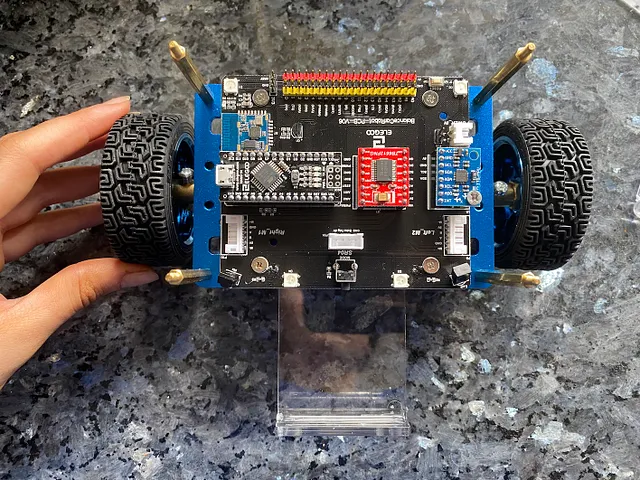
\includegraphics[width=0.7\linewidth]{assets/assembly1}
	\caption{Assembling arduino nano, motor driver, mpu6050 sensor and motors on the robot base.}
	\label{fig:assembly1}
\end{figure}

\begin{figure}[H]
	\centering
	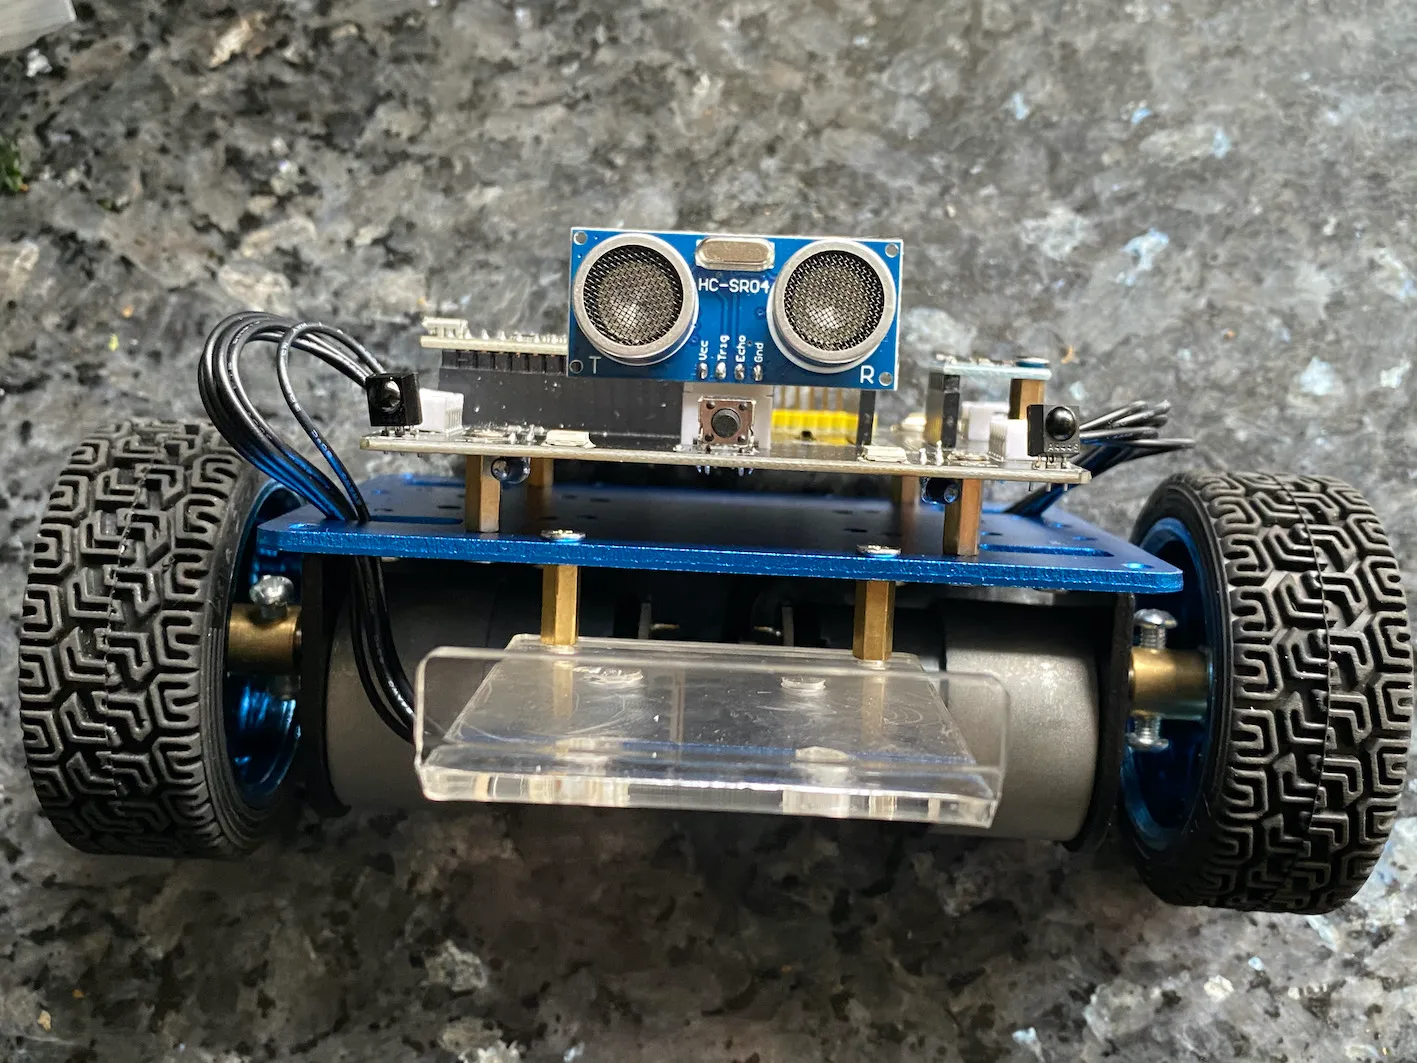
\includegraphics[width=0.7\linewidth]{assets/assembly2}
	\caption{Attaching the ultrasonic sensor.}
	\label{fig:assembly2}
\end{figure}

\begin{figure}[H]
	\centering
	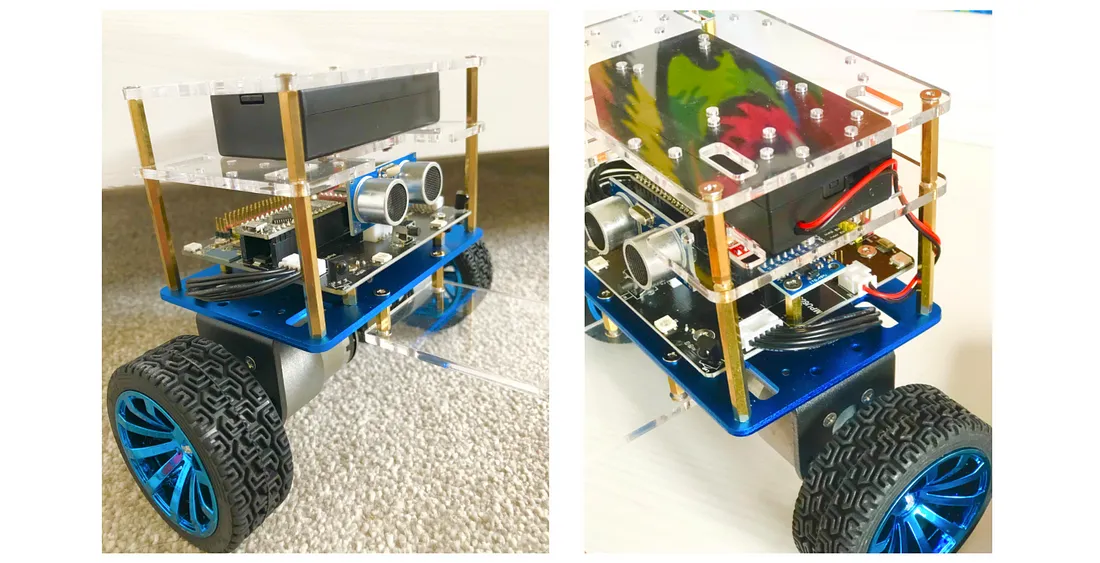
\includegraphics[width=0.7\linewidth]{assets/assembly3}
	\caption{Final Assembly.}
	\label{fig:assembly3}
\end{figure}
	\section{TerraRanger Multiflex}
The TeraRanger Multiflex is a modular Time-of-Flight (ToF) (shown in Fig.~\ref{fig:terraMount}) sensor array designed for robotics applications, including SLAM and maze-solving. The system includes eight ToF sensors, a Multiflex Hub, flex cables, and connectors, enabling flexible deployment \cite{terra_mount}.

\begin{figure}[H]
	\centering
	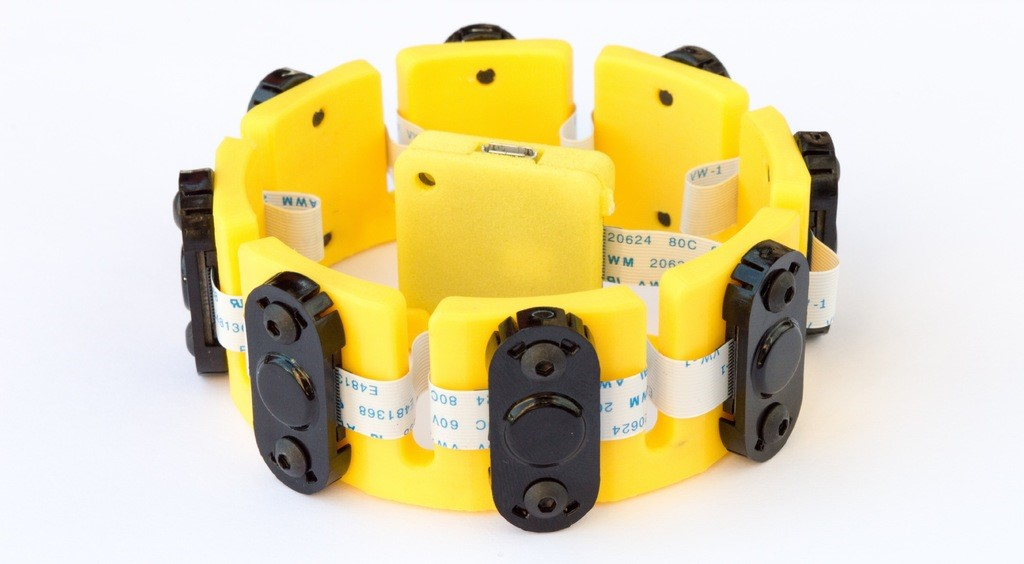
\includegraphics[height=6cm]{assets/terraRangerMultiplex.jpg}
	\caption{TeraRanger Multiflex circular mount \cite{terra_mount}.}
	\label{fig:terraMount}
\end{figure}

\textbf{Key Features and Considerations}
\begin{itemize}
	\item \textbf{Compact and Modular Design}: Each sensor is enclosed in a polycarbonate cover and can be mounted using M3 screws.
	\item \textbf{Safe Laser Emission}: The sensors utilize a low-power laser emitter; optical modifications are not recommended.
	\item \textbf{Stable Power Requirements}: Operates at 5V ±0.25V with minimal ripple and noise.
	\item \textbf{Reliable Connectivity}: Utilizes a 7-pin Hirose DF13 connector for UART/I2C communication; designed for robust vibration-resistant connections.
	\item \textbf{Mounting Precautions}: Avoid exposure to heat, dust, and strong electromagnetic fields for optimal performance.
\end{itemize}

\subsection{Connector and Data Interfaces}
\begin{figure}[H]
	\centering
	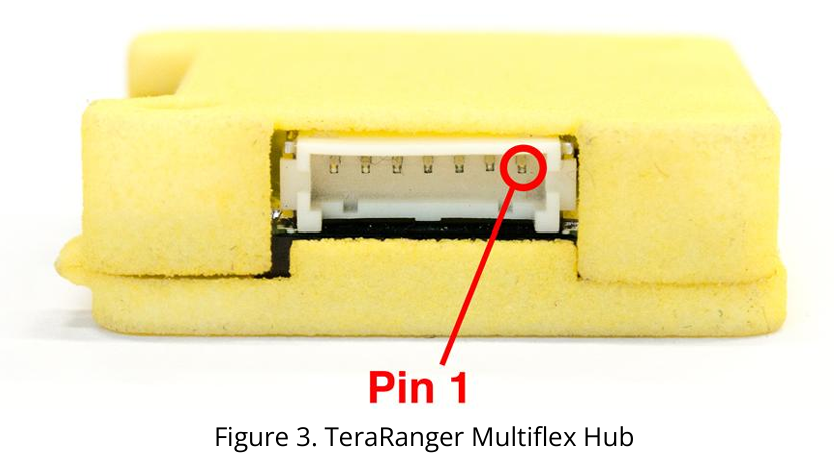
\includegraphics[height=3cm]{assets/TerraRangerMultflexHubPinout.png}
	\caption{TeraRanger Multiflex Hub pinout \cite{terra_mount}.}
	\label{fig:terraPinout}
\end{figure}

The \textbf{TeraRanger Multiflex Hub} connects to external equipment via a \textbf{7-pin Hirose DF13 connector} (female part: \textbf{DF13-7S-1.25C}). A compatible connector cable is included in the package. The pin configuration is as follows:

\begin{table}[H]
	\centering
	\begin{tabular}{|c|l|}
		\hline
		\textbf{Pin} & \textbf{Function} \\
		\hline
		7   & GND \\
		6   & RX Serial In (UART) \\
		5   & TX Serial Out (UART) \\
		4   & Interrupt Pin \\
		3   & SDA (I2C) \\
		2   & SCL (I2C) \\
		1   & 5 V Power Supply \\
		\hline
	\end{tabular}
	\caption{TeraRanger Multiflex Hub connector pinout}
	\label{tab:multiflex_pinout}
\end{table}

\subsection{UART Data Interface (Default)}
The \textbf{UART interface} operates at \textbf{3.3V output levels} (accepting inputs from \textbf{3.3V to 5V}). To connect the hub to a computer, a \textbf{USB-to-serial adapter} (e.g., FTDI breakout board) should be used. The default UART configuration is:

\begin{itemize}
	\item \textbf{Baud Rate:} 115200 bit/s
	\item \textbf{Data Bits:} 8
	\item \textbf{Parity:} None
	\item \textbf{Stop Bits:} 1
\end{itemize}

\subsection{I2C Data Interface}
The \textbf{I2C interface} allows the hub to function as a slave device, connecting to an I2C master. The default \textbf{I2C base address} is \textbf{0x55}, and only one \textbf{TeraRanger Multiflex} can be used per I2C bus. The signal levels are \textbf{3.3V}, and the \textbf{maximum bus speed is 400 kHz}. Integrated \textbf{1.5k Ohm pull-up resistors} ensure proper bus communication.

\subsection{USB Interface}
A \textbf{micro-USB} port provides both \textbf{power and data communication}. On \textbf{Linux and macOS}, the hub appears as a \textbf{virtual COM port} without additional drivers. On \textbf{Windows}, a driver must be installed from:  

\begin{center}
	\url{http://www.st.com/en/development-tools/stsw-stm32102.html}
\end{center}

After installation, reconnect the device to enable the COM port. The communication settings remain \textbf{115200-8N1}.


	\section{Maze Solving Alogrithms}
Maze Solving Using Right-then-Left and Left-then-Right Navigation

Maze solving is a fundamental capability for autonomous mobile robots, requiring efficient navigation strategies to explore and determine the optimal path to an exit or target. The two-wheeled self-balancing robot employs two heuristic-based approaches for maze traversal: Right-then-Left (RTL) navigation and Left-then-Right (LTR) navigation. Both methods operate under the assumption that the maze consists of walls and corridors, where the robot continuously follows one side until reaching a dead-end or an unexplored path.

\subsection{Right-Then-Left (RTL) Navigation}
In the RTL approach, the robot prioritizes right turns whenever a choice is available. If no right turn is possible, it proceeds forward. If forward movement is blocked, it turns left. If no left turn is possible, it executes a U-turn. The algorithm follows these steps:
\begin{itemize}
	\item If a right turn is available, turn right.
	\item If a right turn is not possible, move straight.
	\item If a dead-end is encountered, turn left.
	\item If all directions are blocked, perform a U-turn.
\end{itemize}

\textbf{Dead-End Handling}:
The robot detects dead-ends using sensor feedback and reverses until a possible turn is detected.
It switches to the left wall when navigating out of loops or returning from an incorrect path.

\textbf{Cycle Detection and Backtracking}:
To prevent getting stuck in loops, the robot stores visited junctions and alters its strategy if it encounters a repeated state.
If a previously visited path is identified, it backtracks and prioritizes alternative routes.

\subsection{Left-Then-Right (LTR) Navigation}
The LTR approach mirrors the RTL method but prioritizes left turns instead of right turns. This strategy is useful in mazes where a left-biased path leads to a shorter exit route. The algorithm follows these steps:
\begin{itemize}
	\item If a left turn is available, turn left.
	\item If a left turn is not possible, move straight.
	\item If a dead-end is encountered, turn right.
	\item If all directions are blocked, perform a U-turn.
\end{itemize}

\textbf{Dead-End Handling and Backtracking}:
Similar to RTL, the robot maintains a memory of visited locations to avoid infinite loops.
If an already explored junction is reached again, the algorithm forces a deviation.

\textbf{Cycle Detection and Backtracking}:
To prevent getting stuck in loops, the robot stores visited junctions and alters its strategy if it encounters a repeated state.
If a previously visited path is identified, it backtracks and prioritizes alternative routes.

\subsection{Algorithm Implementation}
Both RTL and LTR methods can be implemented using a combination of wall-following, decision-tree logic, and sensor-based navigation. The robot uses:

Infrared or ultrasonic sensors to detect walls and available paths.
Odometry and IMU data to maintain orientation and track previously visited locations.
A finite-state machine (FSM) to switch between different navigation states.

A pseudo-code representation of both strategies is as follows:
\begin{lstlisting}[style=cppstyle2]
void navigate_maze_RTL() {
	if (right_available()) {
		turn_right();
	} else if (forward_available()) {
		move_forward();
	} else if (left_available()) {
		turn_left();
	} else {
		u_turn();
	}
}
\end{lstlisting}

\begin{lstlisting}[style=cppstyle2]
void navigate_maze_LTR() {
	if (left_available()) {
		turn_left();
	} else if (forward_available()) {
		move_forward();
	} else if (right_available()) {
		turn_right();
	} else {
		u_turn();
	}
}
\end{lstlisting}
	\section{Results}
		%\include{challenges_and_limitaRtions.tex}
	\section{Future Work and Improvements}

While the current implementation of the two-wheeled self-balancing robot achieved significant milestones, several areas for future improvement were identified.

\subsection{Enhanced Control Algorithms}
Exploring advanced control techniques such as adaptive control and machine learning-based approaches could further enhance the robot's stability and performance.

\subsection{Autonomous Navigation}
Integrating additional sensors like LiDAR and implementing SLAM (Simultaneous Localization and Mapping) algorithms would enable the robot to navigate autonomously in complex environments.

\subsection{Mobile App Development}
Developing a dedicated mobile application with enhanced features and a more user-friendly interface would improve the overall user experience.

\subsection{Extended Battery Life}
Investigating alternative power sources or more efficient battery management systems could extend the robot's operational time.
	\begin{appendices}
\section{Calculation of the system's transfer functions} \label{appendix:tf-calculations}
To simplify the model, we assume that it can be represented as an inverted pendulum attached to a cart. Calculations about inverted pendulum attached to a cart is common and can be found on several websites on the internet, this will help ensure
that these calculations are correct. The following calculations were inspired by MathWorks \cite{matlab_inverted_pendulum}.

\begin{figure}[h]
	\centering
	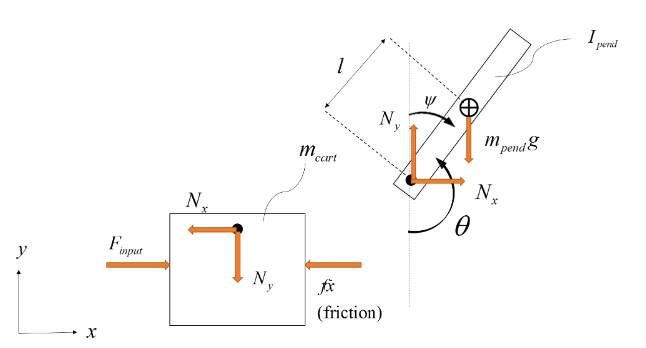
\includegraphics[height=6cm]{assets/FBD-inverted-pendulum.png}
	\caption{\label{fig:fbd}Exposure of the simplified system with cart and pendulum \cite{10193276}.}
\end{figure}


\subsection{Equation for the cart}
The only equation needed from the cart is the one who sums the forces in the x direction
\begin{equation}
F_{input} = m_{cart} \ddot{x} + f \dot{x} + N_x 
\end{equation} 

where \(F_{input}\) is an applied force, \(m_{cart}\) is the mass of the cart, f is a constant of friction and \( N_x \) is the contact force in the axis between cart and pendulum in x-direction (see Fig.~\ref{fig:fbd}).


\subsection{Equation for the the pendulum}
The sum of forces in the x direction on the pendulum is
\begin{equation}
	N_x = m_{pend} \ddot{x} + m_{pend} l \ddot{\theta} \cos \theta - m_{pend} l \dot{\theta}^2 \sin \theta \label{eq:force_x}
\end{equation}
where $m_{pend}$ is the mass and $l$ is the distance to the center of mass. Variable $\theta$ is the angle between a vertical line and the pendulum. See Figure for details.

The sum of all forces perpendicular to the pendulum is
\begin{equation}
	N_y \sin \theta + N_x \cos \theta = m_{pend} g \sin \theta - m_{pend} l \ddot{\theta} + m_{pend} \dot{\theta}^2 \cos \theta \label{eq:force_perp}
\end{equation}
where $N_y$ is the force in the y direction and $g$ is the gravity constant.

Summarizing the torque acting on the center of the pendulum gives the following equation
\begin{equation}
	- N_y l \sin \theta - N_x l \cos \theta = I_{pend} \ddot{\theta} \label{eq:torque}
\end{equation}
where $I_{pend}$ is the moment of inertia of the pendulum.



=\subsection{Combining the equations} \label{appendix:graph}
Insert equation (\ref{eq:force_x}) in (\ref{eq:force_perp}) gives the following equation
\begin{equation}
	F_{input} = (m_{cart} + m_{pend}) \ddot{x} + f \dot{x} + m_{pend} l \ddot{\theta} \cos \theta - m_{pend} l \dot{\theta}^2 \sin \theta \label{eq:combined_force}
\end{equation}
Combine equations (\ref{eq:torque}) and (\ref{eq:combined_force})
\begin{equation}
	(I_{pend} + m_{pend} l^2) \ddot{\theta} + m_{pend} g l \sin \theta = -m_{pend} l \ddot{x} \cos \theta \label{eq:combined_torque}
\end{equation}


\subsection{Linearising the equations}
Equation (\ref{eq:linearized_force}) and (\ref{eq:linearized_torque}) is necessary to get transfer functions for the position $x$ and the angle deviation $\psi$. To compute the transfer functions the equations need to be linearized. A proper equilibrium point would be when the pendulum is in upright position. The angle will represent the deviation of the pendulum from the equilibrium. The following approximations for small deviations will be used in the nonlinear equations (\ref{eq:combined_force}) and (\ref{eq:combined_torque}).

\begin{equation}
	\cos \theta = \cos(\pi + \psi) \approx -1 \label{eq:cos_approx}
\end{equation}

\begin{equation}
	\sin \theta = \sin(\pi + \psi) \approx -\psi \label{eq:sin_approx}
\end{equation}

\begin{equation}
	\dot{\theta}^2 = \dot{\psi}^2 \approx 0 \label{eq:theta_dot_approx}
\end{equation}

Linearization with (\ref{eq:cos_approx}), (\ref{eq:sin_approx}) and (\ref{eq:theta_dot_approx}) in (\ref{eq:combined_force}) and (\ref{eq:combined_torque}) leads to the following approximated linear equations where $F_{input}$ has been substituted for the more general control effort $u_{input}$.

\begin{equation}
	(I_{pend} + m_{pend} l^2) \ddot{\psi} - m_{pend} g l \psi = m_{pend} l \ddot{x} \label{eq:linearized_torque}
\end{equation}

\begin{equation}
	u_{input} = (m_{cart} + m_{pend}) \ddot{x} + f \dot{x} - m_{pend} l \ddot{\psi} \label{eq:linearized_force}
\end{equation}


\subsection{Laplace transform}
To obtain the transfer functions, equations (\ref{eq:linearized_torque}) and (\ref{eq:linearized_force}) is transformed to the Laplace domain, the transformation is here denoted by upper case letters.

\begin{equation}
	(I_{pend} + m_{pend} l^2) \Psi(s) s^2 - m_{pend} g l \Psi(s) = m_{pend} l X(s) s^2 \label{eq:laplace_torque}
\end{equation}

\begin{equation}
	U_{input}(s) = (m_{cart} + m_{pend}) X(s) s^2 + f X(s) s - m_{pend} l \Psi(s) s^2 \label{eq:laplace_force}
\end{equation}

A transfer function is a relationship between a single input and a single output, therefore it is needed to solve $X(s)$ from equation (\ref{eq:laplace_torque}).

\begin{equation}
	X(s) = \left[ \frac{I_{pend} + m_{pend} l^2}{m_{pend} l} - \frac{g}{s^2} \right] \Psi(s) \label{eq:X_solution}
\end{equation}

Substitute (\ref{eq:X_solution}) into (\ref{eq:laplace_force}) gives

\begin{equation}
\begin{split}
	U_{input}(s) = & (m_{cart} + m_{pend}) \left[ \frac{I_{pend} + m_{pend} l^2}{m_{pend} l} - \frac{g}{s^2} \right] \Psi(s) s^2  \\ 
	& + f \left[ \frac{I_{pend} + m_{pend} l^2}{m_{pend} l} - \frac{g}{s^2} \right] \Psi(s) s - m_{pend} l \Psi(s) s^2 
\end{split}
	\label{eq:U_substituted}
\end{equation}

If equation (\ref{eq:U_substituted}) is rearranged we get the transfer function $G_\Psi(s)$ as the relation between $\Psi(s)$ and $U_{input}(s)$ as seen in (\ref{eq:transfer_function}).

\begin{equation}
	G_\Psi(s) = \frac{\Psi(s)}{U_{input}(s)} \label{eq:transfer_function}
\end{equation}

\begin{equation}
	\Psi(s) = \underbrace{\frac{\frac{m_{pend} l}{q} s}{s^3 + \frac{f(I_{pend} + m_{pend} l^2)}{q} s^2 - \frac{(m_{cart} + m_{pend}) m_{pend} g l}{q} s - \frac{f m_{pend} g l}{q}}}_{G_\Psi(s)} U_{input}(s) \label{eq:transfer_function_psi}
\end{equation}

where
\begin{equation}
	q = [(m_{cart} + m_{pend})(I_{pend} + m_{pend} l^2) - (m_{pend} l)^2] \label{eq:q_definition}
\end{equation}

The transfer function $G_x(s)$ that describes the cart position $X(s)$ looks as
\begin{equation}
	X(s) = \underbrace{\frac{\frac{(I_{pend} + m_{pend} l^2) s^2 - g m_{pend} l}{q}}{s^4 + \frac{f(I_{pend} + m_{pend} l^2)}{q} s^3 - \frac{(m_{cart} + m_{pend}) m_{pend} g l}{q} s^2 - \frac{f m_{pend} g l}{q} s}}_{G_x(s)} U_{input}(s) \label{eq:transfer_function_x}
\end{equation}


\subsection{State Space Modelling}
It is possible to present the system in state space form. The matrix form is
\begin{equation}
	\begin{bmatrix}
		\dot{x} \\
		\ddot{x} \\
		\dot{\psi} \\
		\ddot{\psi}
	\end{bmatrix} = A \begin{bmatrix}
		x \\
		\dot{x} \\
		\psi \\
		\dot{\psi}
	\end{bmatrix} + B u_{input} \label{eq:state_space}
\end{equation}
where
\begin{equation}
	A = \begin{bmatrix}
		0 & 1 & 0 & 0 \\
		0 & \frac{-(I_{pend} + m_{pend} l^2) f}{I_{pend} (m_{cart} + m_{pend}) + m_{cart} m_{pend} l^2} & \frac{m_{pend}^2 g l^2}{I_{pend} (m_{cart} + m_{pend}) + m_{cart} m_{pend} l^2} & 0 \\
		0 & 0 & 0 & 1 \\
		0 & \frac{-m_{pend} l f}{I_{pend} (m_{cart} + m_{pend}) + m_{cart} m_{pend} l^2} & \frac{m_{pend} g l (m_{cart} + m_{pend})}{I_{pend} (m_{cart} + m_{pend}) + m_{cart} m_{pend} l^2} & 0
	\end{bmatrix} \label{eq:state_matrix_A}
\end{equation}
\begin{equation}
	B = \begin{bmatrix}
		0 \\
		\frac{I_{pend} + m_{pend} l^2}{I_{pend} (m_{cart} + m_{pend}) + m_{cart} m_{pend} l^2} \\
		0 \\
		\frac{m_{pend} l}{I_{pend} (m_{cart} + m_{pend}) + m_{cart} m_{pend} l^2}
	\end{bmatrix} \label{eq:state_matrix_B}
\end{equation}
\begin{equation}
	C = \begin{bmatrix}
		1 & 0 & 0 & 0 \\
		0 & 0 & 1 & 0
	\end{bmatrix} \label{eq:state_matrix_C}
\end{equation}

It is possible to present the system in state space form. The matrix form, ignoring position and velocity states, is:

\begin{equation}
	\begin{bmatrix}
		\dot{\psi} \\
		\ddot{\psi}
	\end{bmatrix} = A \begin{bmatrix}
		\psi \\
		\dot{\psi}
	\end{bmatrix} + B u_{input} \label{eq:reduced_state_space}
\end{equation}

where

\begin{equation}
	A = \begin{bmatrix}
		0 & 1 \\
		\frac{m_{pend} g l (m_{cart} + m_{pend})}{I_{pend} (m_{cart} + m_{pend}) + m_{cart} m_{pend} l^2} & 0
	\end{bmatrix} \label{eq:reduced_state_matrix_A}
\end{equation}

\begin{equation}
	B = \begin{bmatrix}
		0 \\
		\frac{m_{pend} l}{I_{pend} (m_{cart} + m_{pend}) + m_{cart} m_{pend} l^2}
	\end{bmatrix} \label{eq:reduced_state_matrix_B}
\end{equation}

\begin{equation}
	C = \begin{bmatrix}
		1 & 0
	\end{bmatrix} \label{eq:state_matrix_C}
\end{equation}



\section{Calculation for Kalman Filter} \label{appendix:B}
\subsection{Initialization}
Defining an initialization according to:
\begin{equation}
	P(0) = \mathbf{E}(\Delta\underline{x}(0) \Delta\underline{x}^T(0))  \label{eq:eq}
\end{equation}
where $P(0)$ is the initial covariance matrix, presenting the expected uncertainty in the initial state estimate. It is calculated based on the expected error in the initial state.


\subsection{Optimal Kalman Gain}
We can find optimal Kalman gain matrix $\underline{K}(t)$ as following:
\begin{equation}
	\underline{K}(t) = P(t) \underline{C}^T(t) R^{-1}  \label{eq:eq}
\end{equation}
It determines much the state estimate should be adjusted based on the measurement residual. It balances the uncertainty in the state estimate and the measurement noise.


\subsection{Time-Discrete Kalman Filter}
The time-discrete Kalman filter equations are expressed as:
\begin{equation}
	\begin{aligned}
		\underline{x}_{k} &= \underline{A} \underline{x}_{k-1} + \underline{B} \underline{u}_{k} + \underline{d}_{k-1} \\
		\underline{y}_{k} &= \underline{C} \underline{x}_{k} + \underline{n}_{k}  \label{eq:eq}
	\end{aligned}
\end{equation}

where, 
\begin{itemize}
	\item $\underline{x}_k$: This is the state vector at time step $k$.
	\item $\underline{B}$: This is the control input matrix, which relates the control inputs $\underline{u}_k$ to the state.
	\item $\underline{y}_k$: This is the measurement vector at time step $k$.
	\item $\underline{d}_{k-1}$: This represents process noise at the previous time step.
	\item $\underline{n}_k$: This represents measurement noise at time step $k$.
\end{itemize}


\subsection{Estimated states:}
The estimated states are given by:
\begin{equation}
	\begin{aligned}
		\underline{\hat{x}}_{k} &= \underline{A} \  \underline{\hat{x}}_{k-1} + \underline{B} \ \underline{u}_{k} + \underline{d}_{k-1} \\
		\underline{\hat{y}}_{k} &= \underline{C} \ \underline{\hat{x}}_{k} + \underline{n}_{k}  \label{eq:eq}
	\end{aligned}
\end{equation}


\subsection{Discrete State Equation}
The state-space representation of the system is given by:
\begin{equation}
	\begin{aligned}
		\underline{\dot{x}}(t) = \underline{A}.\underline{x}(t) + \underline{B}.\underline{u}(t) \\
		\underline{y}(t) = \underline{C}.\underline{x}(t) + \underline{D}.\underline{u}(t)  \label{eq:eq}
	\end{aligned}
\end{equation}
where the components of the State-Space Representation are,
\begin{itemize}
	\item \textbf{State Vector} $\mathbf{\underline{x}(t)}$: This vector encapsulates the internal state of the system at time t. It this case, it is defined as $\mathbf{x}_{k} = \begin{bmatrix} \text{angle} \\ \text{q\_bias} \end{bmatrix}$. Where \text{angle} represents the measured angle of the system, while \text{q\_bias} denotes the bias of the gyroscope.
	
	\item \textbf{State Transition Matrix} $\underline{\mathbf{A}}$: This matrix describes how the state evolves over time. It is defined as: $\mathbf{A}_k = \begin{bmatrix} 1 & -dt \\ 0 & 1 \end{bmatrix}$ The first row indicates that the angle is updated based on its previous value and the time step $dt$, while the second row shows that the gyroscope bias remains constant in this model.
	
	\item \textbf{Control Input Matrix} $\underline{\mathbf{B}}$: This matrix relates the control inputs to the state. In this case, it is defined as:
	$\mathbf{B}_k = 0$. This indicates that there are no direct control inputs affecting the state in this model.
	
	\item \textbf{Measurement Matrix} $\underline{\mathbf{C}}$: This matrix maps the state vector to the measurement output. It is defined as: $\mathbf{C}_k = \begin{bmatrix} 1 & 0 \end{bmatrix}$. This means that the measurement output directly reflects the angle, with no contribution from the gyroscope bias.
	
	\item \textbf{Feedforward Matrix} $\underline{\mathbf{D}}$: This matrix relates the control input directly to the measurement output. In this case, it is defined as: $\mathbf{D}_k = 0$. This indicates that there is no direct influence of the control input on the measurement output.	
\end{itemize}


\subsection{Measurement Noise Covariance Matrix $\mathbf{R}$}
The measurement noise variance for the angle sensor is defined as:
\begin{equation} \mathbf{R}_{k} = R_{angle} \end{equation}


\subsection{Process/System Noise Covariance Matrix $\mathbf{Q}$}
The process noise covariance matrix is given by:
\begin{equation}
	\mathbf{Q} = \begin{bmatrix} Q_{\text{angle}} & 0 \\ 0 & Q_{\text{gyro bias}} \end{bmatrix} * \Delta t  \label{eq:eq}
\end{equation}


\subsection{State Covariance Matrix $\mathbf{P}$}
The state covariance matrix is represented as:
\begin{equation}
	\mathbf{P}_k = \begin{bmatrix} P_{00} & P_{01} \\ P_{10} & P_{11} \end{bmatrix}  \label{eq:eq}
\end{equation}
\begin{itemize}
	\item $P_{00}$ represents the uncertainty in the angle estimate.
	\item $P_{11}$ represents the uncertainty in the gyroscope bias estimate.
	\item $P_{01} = P_{10}$ represent the covariance between the angle and gyroscope bias.
\end{itemize}


\subsection{Kalman Gain $\mathbf{K}$:}
The Kalman gain is defined as:
\begin{equation}
	\mathbf{K}_k = \begin{bmatrix} K_{0} \\ K_{1} \end{bmatrix}  \label{eq:eq}
\end{equation}


\subsection{Estimated states}
The estimated states are updated as follows:
\begin{equation}
	\theta_{measured} = \theta_{measured} + (\omega_{measured} - \omega_{bias}) * \Delta t  \label{eq:eq}
\end{equation}


\subsection{Error Calculation}
The error in the angle estimate is calculated as:
\begin{equation} 
	\theta_{error} = \theta_{measured} - \theta_{desired}  \label{eq:eq} 
\end{equation}

\subsection{Time Update (prediction)}
The time update for the state covariance matrix is given by:
\begin{equation}
	\mathbf{P}_k = \begin{bmatrix} P_{00} & P_{01} \\ P_{10} & P_{11} \end{bmatrix}  \label{eq:eq}
\end{equation}
The matrix $P$ reflects the uncertainties in the angle estimate ($P_{00}$), the gyroscope bias ($P_{11}$), and the cross-covariance terms ($P_{01}$, $P_{10}$).


\subsection{Initialization}
The initial state covariance matrix is defined as:
\begin{equation}
	\mathbf{P}_0 = \begin{bmatrix} 1 & 0 \\ 0 & 1 \end{bmatrix}  \label{eq:eq}
\end{equation}
The prediction step for the covariance matrix is:
\begin{equation}
	\mathbf{P}_k = \mathbf{A} \mathbf{P}_{k-1} \mathbf{A^T} + \mathbf{Q}  \label{eq:eq}
\end{equation}

This expands to:
\begin{equation}
	\mathbf{P}_k = \begin{bmatrix} P_{00}^- + [(Q_{\text{angle}} - P_{01}^- - P_{10}^-)*\Delta t]  &  P_{01}^- - (P_{11}^-*\Delta t)  
		\\ P_{10}^- - (P_{11}^-*\Delta t)  &  P_{11}^- + (Q_{\text{gyro bias}}*\Delta t) \end{bmatrix}  \label{eq:eq}
\end{equation}


\subsection{Kalman Gain Calculation}
The Kalman gain $\underline{K}_{k}$ is computed as:
\begin{equation}
	\begin{aligned}
		\underline{K}_{k} &= \underline{P}_{k}^- \ \underline{C}^T ( \underline{C} \ \underline{P}_{k}^-\ \underline{C}^T  +\underline{R})^{-1} \\
		\\
		&= 
		\begin{bmatrix} P_{00} & P_{01} \\ P_{10} & P_{11} \end{bmatrix} \begin{bmatrix} 1 \\ 0 \end{bmatrix}
		\left(
		\begin{bmatrix} 1 & 0 \end{bmatrix} 
		\begin{bmatrix} P_{00} & P_{01} \\ P_{10} & P_{11} \end{bmatrix}  
		\begin{bmatrix} 1 \\ 0 \end{bmatrix} 
		+ R_{angle}
		\right)^{-1} \\ \\
		&= 
		\begin{bmatrix} P_{00} \\ P_{10}\end{bmatrix}
		\left(
		P_{00}  
		+ R_{angle}
		\right)^{-1} \\ \\
		\mathbf{K}_k &= \begin{bmatrix} \frac{ P_{00} }{ P_{00}  
				+ R_{angle}} \\ \frac{ P_{10} }{ P_{00}  
				+ R_{angle}} \end{bmatrix}
	\end{aligned}  \label{eq:eq}
\end{equation}

\subsection{Measurement Update (Correction)}
The measurement update for the state covariance matrix is given by:
\begin{equation}
	\begin{aligned}
		\underline{P}_{k} &= \ (\underline{I} - \underline{K}_{k} \ \underline{C}) \ \underline{P}_{k}^- \\ 
		&= \ \left( \begin{bmatrix} 
			1 & 0 \\ 
			0 & 1 
		\end{bmatrix}
		- 
		\begin{bmatrix} 
			K_{0} \\  
			K_{1} 
		\end{bmatrix} 
		\begin{bmatrix} 
			1 & 0 
		\end{bmatrix}  
		\right) 
		\begin{bmatrix}
			P_{00} & P_{01} \\ 
			P_{10} & P_{11} 
		\end{bmatrix} 
		&=  
		\begin{bmatrix} 
			1 - K_{0} & 0 \\ 
			-K_{1} & 1 
		\end{bmatrix} 
		\begin{bmatrix} 
			P_{00} & P_{01} \\ 
			P_{10} & P_{11} 
		\end{bmatrix}  \\ \\
		&= 
		\begin{bmatrix} 
			P_{00} - K_{0} \cdot P_{00} & P_{01} - K_{0} \cdot P_{01} \\
			P_{10} - K_{1} \cdot P_{00} & P_{11} - K_{1} \cdot P_{01} \\
		\end{bmatrix}  \label{eq:eq}
	\end{aligned}
\end{equation}
\section{Third Appendix} \label{appendix:C}

\end{appendices}
	\printbibliography

\end{document}